
\begin{center}\noindent
{\bf \Large Online Appendix}\\ \vspace{3\baselineskip}
{\bf \Large Loan Guarantees in a Crisis:\\An Antidote to a Credit Crunch?}\\ \vspace{3\baselineskip}
%{\bf \Large W. Blake Marsh and Padma Sharma}
\end{center}

\begin{onehalfspace}
\clearpage
\pagebreak
\appendix
\renewcommand{\thesection}{\Alph{section}}

%% Section A
\section{Simulation Study\label{onappx_sec:sim_study}}
\setcounter{table}{0}
\renewcommand{\thetable}{A.\arabic{table}}
Table \ref{sim_results} presents the results of the simulation study that demonstrate that we can recover true parameter values with or without exclusion restrictions. However, we obtain more precise estimates with exclusion restrictions. We set the following priors under the two specifications: $\theta \sim \mathcal{N}(0, 10\times\mathbf{I})$, $\Omega_{p} \sim \mathcal{IW}(7,3\times\mathbf{I}_{4})$, and $\Omega_{np} \sim \mathcal{IW}(7,3\times\mathbf{I}_{3})$ where $\theta = [\gamma_{1}, \gamma_{2}, \delta, \boldsymbol{\beta}]$, and $\boldsymbol{\beta} = \{\beta_{1},\beta_{2},\beta_{3},\beta_{4}\}$. 
% Table generated by Excel2LaTeX from sheet 'Final'
\begin{table}[htbp]
  \centering
  \caption{Simulation Results\label{sim_results}}
    \resizebox{1\textwidth}{!}{
   \begin{threeparttable}
    \begin{tabular}{lrlrl}
    \hline\hline
          & \multicolumn{2}{c}{No exclusion} & \multicolumn{2}{c}{Exclusion} \\
          & \multicolumn{1}{l}{True values} & \multicolumn{1}{l}{95\% credibility interval} & \multicolumn{1}{l}{True values} & 95\% credibility interval \\
          \hline
    $\beta_{11}$ & -0.1  & [-0.23, 0.08] & -0.1  & [-0.16, -0.06] \\
    $\beta_{12}$ & -0.2  & [-0.37, -0.14] & -0.2  & [-0.21, -0.1] \\
    $\beta_{13}$ & 0.1   & [-0.07, 0.15] & 0.1   & [0.08, 0.13] \\
    $\beta_{14}$ & 0.2   & [0.06, 0.27] & 0.2   & [0.16, 0.22] \\
    $\beta_{21}$ & 1     & [0.8, 1.95] & 1     & [0.88, 1.12] \\
    $\beta_{22}$ & 0.5   & [0.43, 0.72] & 0.5   & [0.47, 0.51] \\
    $\beta_{23}$ & -0.6  & [-0.67, -0.43] & -0.6  & [-0.62, -0.57] \\
    $\beta_{24}$ & -1    & [-1.13, -0.88] & -1    & [-1.03, -0.96] \\
    $\beta_{31}$ & 2     & [1.37, 2.58] & 2     & [1.89, 2.12] \\
    $\beta_{32}$ & -3    & [-3.21, -2.66] & -3    & [-3.05, -2.99] \\
    $\beta_{33}$ & 2.5   & [2.31, 2.69] & 2.5   & [2.46, 2.52] \\
    $\beta_{34}$ & 4     & [3.77, 4.29] & 4     & [3.94, 4.03] \\
    $\beta_{41}$ & -2    & [-2.58, -1.67] & -2    & [-2.37, -1.66] \\
    $\beta_{42}$ & 1.5   & [1.42, 1.65] & 2     & [1.94, 2.02] \\
    $\beta_{43}$ & -3    & [-3.09, -2.85] & -3    & [-3.08, -2.95] \\
    $\Omega_{12}$ & 0.5   & [-0.69, 0.6] & 0.5   & [0.33, 0.57] \\
    $\Omega_{22}$ & 0.8   & [0.57, 1.06] & 0.8   & [0.69, 0.86] \\
    $\Omega_{13}$ & 0.5   & [-0.34, 1.08] & 0.5   & [0.45, 0.67] \\
    $\Omega_{23}$ & -0.1  & [-0.82, -0.12] & -0.1  & [-0.14, -0.04] \\
    $\Omega_{33}$ & 0.75  & [0.7, 1.53] & 0.75  & [0.69, 0.87] \\
    $\Omega_{14}$ & -0.2  & [-0.82, 0.5] & -0.2  & [-0.72, 0.3] \\
    $\Omega_{44}$ & 0.8   & [0.74, 1.28] & 0.8   & [0.77, 1.11] \\
    \hline\hline
    \end{tabular}%
   \begin{tablenotes}
        \footnotesize \item Note: The 95\% credibility intervals in brackets. The results are based on 11,000 MCMC draws with a burn-in of 1000. The specification of ``Exclusion" consists of an instrument in the selection equation.   The specification of ``No exclusion" consists of no instruments in the selection equation.   
    \end{tablenotes}
\end{threeparttable}
    }
\end{table}%


\clearpage




%% Section B
\section{Categorization of COVID-sensitive industries\label{onappx_sec:employment}}
\setcounter{figure}{0}
\renewcommand{\thefigure}{B.\arabic{figure}}
This appendix presents the sorted declines in employment by NAICS sector bet ween January and April 2020. These sectors are used to determine pre-pandemic county level exposures to COVID as-of 2019:Q4. Bank-market specific COVID exposures are assembled by weighting county exposures by bank deposits. The methodology is taken from \citet{Boyarchenko2020}.

\afterpage{
\begin{landscape}
\begin{figure}[ht]
  \begin{center}
   \caption{Change in employment}
    \includegraphics[angle=270, scale=0.64]{./charts/online_appendix/employment_growth_quartiles.eps}
    \label{cov_sens_ind}
  \end{center}
\footnotesize Chart shows percent change in employment over Jan - Apr 2020 across industries.\\ Source: CES data from the Bureau of Labor Statistics.
\end{figure}
\end{landscape}
}
\clearpage





%% Section C
\section{Additional Participation and Intensity Results\label{onappx_sec:addl_results}}
\setcounter{table}{0}
\renewcommand{\thetable}{C.\arabic{table}}

The tables in this section report the full participation, intensity, and outcome results for the models reported in the paper.

\begin{landscape}
\begin{table}[htbp]
  \centering
  \footnotesize
  \caption{Results for participation and intensity from the Bayesian joint model\label{tab:bayes_jm_app}}
  \resizebox{1.35\textwidth}{!}{
   \begin{threeparttable}
    \begin{tabular}{rcccccc}
    \hline\hline
          & \multicolumn{2}{c}{$\Delta$NIM} & \multicolumn{2}{c}{Non-PPP C\&I Gwth} & \multicolumn{2}{c}{CRE Gwth} \\
          \hline
          &\multicolumn{1}{c}{(1)} & \multicolumn{1}{c}{(2)} & \multicolumn{1}{c}{(3)} & \multicolumn{1}{c}{(4)} & \multicolumn{1}{c}{(5)} & \multicolumn{1}{c}{(6)}\\
                    \hline
          & Part. & Intensity & Part. &  Intensity & Part. & Intensity\\
          \hline
    		\multicolumn{1}{l}{Tech exp. to assets} & -0.08 &       & -0.09 &       & 0.02  &  \\
		& [-0.2, 0.04] &       & [-0.17, -0.01] &       & [-0.07, 0.11] &  \\
		\multicolumn{1}{l}{COVID-affected employment share} &       & 0.04  &       & 0.03  &       & 0.03 \\
		&       & [0.03, 0.05] &       & [0.02, 0.04] &       & [0.02, 0.04] \\
		\multicolumn{1}{l}{ln Assets} & 0.17  & 1.15  & 0.15  & 1.12  & 0.19  & 1.25 \\
		& [0.14, 0.19] & [1.01, 1.29] & [0.13, 0.17] & [0.99, 1.24] & [0.17, 0.21] & [1.12, 1.38] \\
		\multicolumn{1}{l}{CI to assets} & 0.03  & 0.30  & 0.04  & 0.31  & 0.03  & 0.30 \\
		& [0.03, 0.04] & [0.28, 0.33] & [0.03, 0.04] & [0.28, 0.33] & [0.03, 0.04] & [0.27, 0.32] \\
		\multicolumn{1}{l}{Leverage Ratio} & -0.05 & -0.33 & -0.04 & -0.30 & -0.04 & -0.30 \\
		& [-0.06, -0.04] & [-0.38, -0.27] & [-0.05, -0.03] & [-0.36, -0.25] & [-0.05, -0.03] & [-0.36, -0.25] \\
		\multicolumn{1}{l}{Liquid Assets to Assets} & 0.01  & 0.07  & 0.01  & 0.07  & 0.01  & 0.07 \\
		& [0, 0.01] & [0.06, 0.09] & [0, 0.01] & [0.06, 0.09] & [0, 0.01] & [0.06, 0.09] \\
		\multicolumn{1}{l}{ALLL to Total Loans} & -0.02 & 0.13  & -0.03 & 0.09  & -0.02 & 0.12 \\
		& [-0.06, 0.02] & [-0.12, 0.38] & [-0.07, 0.01] & [-0.15, 0.33] & [-0.06, 0.03] & [-0.12, 0.37] \\
		\multicolumn{1}{l}{ROA} & 0.09  & 0.32  & 0.08  & 0.28  & 0.07  & 0.25 \\
		& [0.04, 0.14] & [0.04, 0.6] & [0.03, 0.12] & [0.02, 0.54] & [0.03, 0.12] & [-0.01, 0.52] \\
		\multicolumn{1}{l}{Cases Per 100k} & 0.03  & 0.13  & 0.01  & 0.09  & 0.02  & 0.11 \\
		& [-0.01, 0.06] & [-0.05, 0.31] & [-0.02, 0.04] & [-0.08, 0.27] & [-0.02, 0.05] & [-0.07, 0.28] \\
		\multicolumn{1}{l}{Constant} & -0.98 & -8.70 & -0.82 & -8.38 & -1.25 & -10.01 \\
		& [-1.34, -0.62] & [-10.63, -6.79] & [-1.07, -0.56] & [-10.07, -6.67] & [-1.54, -0.96] & [-11.77, -8.24] \\
          \hline\hline
    \end{tabular}%
    \begin{tablenotes}
        \footnotesize \item Note: The reported values are posterior means of the parameters, and 95\% credibility intervals in brackets. The results are based on 55,000 MCMC draws with a burn-in of 5000.  
    \end{tablenotes}
\end{threeparttable}
    }
\end{table}%
\end{landscape}
\clearpage

\begin{landscape}
\begin{table}[htbp]
	\centering
	\footnotesize
	\caption{Profitability and Loan Growth Outcomes at Participant Banks\label{tab:bayes_jm_2_p_long}}
	\resizebox{1.35\textwidth}{!}{
		\begin{threeparttable}
			\begin{tabular}{lcccc}
				\hline\hline
				& \multicolumn{1}{c}{$\Delta$NIM(bps)}       & \multicolumn{1}{c}{CI Gwth(\%)}      & \multicolumn{1}{c}{Non-PPP CI Gwth(\%)}      & \multicolumn{1}{c}{CRE Gwth(\%)}  \\
				\hline
				& \multicolumn{1}{c}{(1)} & \multicolumn{1}{c}{(2)} & \multicolumn{1}{c}{(3)} & \multicolumn{1}{c}{(4)}\\
				\hline\hline
	$\text{\emph{PPP Loans to Total Loans}}$ & -4.27 & 10.52 & -0.46 & 0.23 \\
	& [-6.03, -2.7] & [9.26, 11.87] & [-1.46, 0.57] & [-0.54, 1.01] \\
	$\ln{Assets}$ & 3.98  & 6.20  & 0.13  & 0.36 \\
	& [2.72, 5.33] & [5.18, 7.19] & [-0.82, 1.04] & [-0.48, 1.2] \\
	$\text{\emph{C\&I to assets}}$ & 0.42  & -7.18 & 0.22  & 0.10 \\
	& [-0.09, 0.97] & [-7.77, -6.63] & [-0.1, 0.54] & [-0.14, 0.34] \\
	$\text{\emph{Leverage Ratio}}$ & -2.48 & -0.23 & -0.09 & 0.28 \\
	& [-3.33, -1.71] & [-0.94, 0.49] & [-0.5, 0.34] & [-0.04, 0.59] \\
	$\text{\emph{Liquid Assets to Assets}}$ & -0.05 & -0.80 & 0.07  & -0.03 \\
	& [-0.2, 0.1] & [-0.99, -0.61] & [-0.02, 0.15] & [-0.1, 0.03] \\
	$\text{\emph{ALLL to Total Loans}}$ & -3.29 & -3.67 & -2.72 & -0.53 \\
	& [-5.28, -1.32] & [-6.2, -1.15] & [-3.65, -1.78] & [-1.23, 0.18] \\
	$\text{\emph{ROA}}$ & -10.48 & 1.38  & -2.12 & -1.84 \\
	& [-12.56, -8.3] & [-1.24, 4.03] & [-3.14, -1.09] & [-2.61, -1.08] \\
	$\text{\emph{Cases Per 100k}}$ & -8.42 & 2.79  & -0.07 & 0.02 \\
	& [-9.76, -7.05] & [0.98, 4.6] & [-0.7, 0.56] & [-0.45, 0.5] \\
	$\text{\emph{Constant}}$ & 0.03  & -0.64 & 2.55  & 0.03 \\
	& [-5.94, 6.06] & [-6.61, 5.35] & [-3.27, 8.41] & [-5.89, 5.91] \\
				\hline\hline
			\end{tabular}%
			\begin{tablenotes}
				\footnotesize \item Note: The reported values are posterior means of the parameters, and 95\% credibility intervals in brackets. The results are based on 55,000 MCMC draws with a burn-in of 5000.  
			\end{tablenotes}
		\end{threeparttable}
	}
\end{table}%
\end{landscape}
\clearpage

\begin{landscape}
\begin{table}[htbp]
	\centering
	\footnotesize
	\caption{Profitability and Loan Growth Outcomes at Non-Participant Banks\label{tab:bayes_jm_2_np_long}}
	\resizebox{1.35\textwidth}{!}{
		\begin{threeparttable}
			\begin{tabular}{lcccc}
				\hline\hline
				& \multicolumn{1}{c}{$\Delta$NIM(bps)}       & \multicolumn{1}{c}{CI Gwth(\%)}      & \multicolumn{1}{c}{Non-PPP CI Gwth(\%)}      & \multicolumn{1}{c}{CRE Gwth(\%)}  \\
				\hline
				& \multicolumn{1}{c}{(1)} & \multicolumn{1}{c}{(2)} & \multicolumn{1}{c}{(3)} & \multicolumn{1}{c}{(4)}\\
				\hline\hline
			$\ln{Assets}$ & -0.91 & -7.47 & -6.64 & -3.72 \\
	& [-4.99, 3.55] & [-8.46, -6.49] & [-7.57, -5.72] & [-4.41, -3.02] \\
	$\text{\emph{C\&I to assets}}$ & -0.10 & 1.42  & -1.86 & -1.07 \\
	& [-1.13, 1.04] & [1.06, 1.79] & [-2.17, -1.56] & [-1.28, -0.87] \\
	$\text{\emph{Leverage Ratio}}$ & -0.26 & 0.84  & 1.98  & 1.06 \\
	& [-1.54, 0.92] & [0.21, 1.46] & [1.36, 2.61] & [0.67, 1.45] \\
	$\text{\emph{Liquid Assets to Assets}}$ & -0.41 & -0.06 & -0.47 & -0.24 \\
	& [-0.68, -0.12] & [-0.23, 0.11] & [-0.64, -0.3] & [-0.36, -0.13] \\
	$\text{\emph{ALLL to Total Loans}}$ & -9.60 & -2.06 & 0.02  & -0.93 \\
	& [-12.19, -6.98] & [-4.6, 0.44] & [-2.42, 2.44] & [-2.55, 0.68] \\
	$\text{\emph{ROA}}$ & -1.54 & -0.03 & -0.39 & 0.27 \\
	& [-5.5, 2.45] & [-3.16, 3.11] & [-3.48, 2.74] & [-1.87, 2.4] \\
	$\text{\emph{Cases Per 100k}}$ & -3.77 & -2.46 & -1.74 & -0.43 \\
	& [-6.83, -0.69] & [-4.75, -0.21] & [-4.02, 0.54] & [-2.03, 1.13] \\
	$\text{\emph{Constant}}$ & -0.60 & -1.27 & 0.68  & -2.00 \\
	& [-6.7, 5.48] & [-7.35, 4.8] & [-5.32, 6.71] & [-7.84, 3.87] \\
				\hline\hline
			\end{tabular}%
			\begin{tablenotes}
				\footnotesize \item Note: The reported values are posterior means of the parameters, and 95\% credibility intervals in brackets. The results are based on 55,000 MCMC draws with a burn-in of 5000.  
			\end{tablenotes}
		\end{threeparttable}
	}
\end{table}%
\end{landscape}

Table \ref{PPPLF_intensity_short} shows the  determinants of banks' participation intensity in the PPPLF from a linear regression model. We focus on the effects of leverage ratio and C\&I exposure, but have considered a range of other controls related to liquidity, profitability, and provisions. Rules that exempted pledged loans from the leverage ratio were an important factor for PPPLF participation. The estimate in column (1) shows that banks with lower leverage ratios were more likely to pledge a larger share of their PPP loans to the PPPLF. Columns (2) and (3) show that the share of C\&I loans on bank balance sheets, both in aggregate, and small C\&I loans in particular enhanced PPPLF participation intensity. In addition, off-balance sheet exposure to C\&I loans were positively associated with PPPLF intensity as noted from the positive coefficients in column (4). This effect of leverage ratio and the share of C\&I loans remain statistically significant even after including all measures jointly in column (5). Banks with substantial C\&I exposure could potentially forestall credit losses, which weigh on capital levels, by lending PPP loans. Exposed banks could then maintain their capital level by financing PPP loans through the PPPLF. Together, the coefficients on leverage and C\&I lending suggest that the exclusion of loans pledged to the PPPLF from the leverage ratio were important in driving bank participation intensity in the liquidity facility.\footnote{Results from a logit model of PPPLF participation also support these conclusions and are available upon request.}  


\begin{table}[!ht]\centering
\def\sym#1{\ifmmode^{#1}\else\(^{#1}\)\fi}
\caption{PPPLF Participation Intensity Determinants\label{PPPLF_intensity_short}}
%\totextwidth{%
\resizebox{.85\textwidth}{!}{
\begin{threeparttable}
\begin{tabular}{l*{10}{c}}
\toprule

            &\multicolumn{1}{c}{(1)}         &\multicolumn{1}{c}{(2)}         &\multicolumn{1}{c}{(3)}         &\multicolumn{1}{c}{(4)}         &\multicolumn{1}{c}{(5)}         \\
\hline\hline
$\text{\emph{Leverage\,\,Ratio}}$&      -0.609\sym{***}&                     &                     &                     &      -0.541\sym{***}\\
            &     (0.098)         &                     &                     &                     &     (0.097)         \\
$\text{\emph{C\&I\,\,to\,\,assets}}$&                     &       0.518\sym{***}&                     &                     &       0.598\sym{***}\\
            &                     &     (0.059)         &                     &                     &     (0.114)         \\
$\text{\emph{Small\,\,C\&I\,\,to\,\,assets}}$&                     &                     &       0.581\sym{***}&                     &      -0.199         \\
            &                     &                     &     (0.090)         &                     &     (0.144)         \\
$\text{\emph{Unused\,\,C\&I\,\,Commitments\,\,to\,\,Assets}}$&                     &                     &                     &       0.605\sym{***}&      -0.017         \\
            &                     &                     &                     &     (0.103)         &     (0.136)         \\
\hline
Observations&       6,940         &       6,940         &       6,940         &       6,940         &       6,940         \\
Adjusted R2 &       0.041         &       0.056         &       0.046         &       0.044         &       0.059         \\
Bank controls      &   Yes         &   Yes         &   Yes         &   Yes         &   Yes         \\
\hline\hline
\end{tabular}
\begin{tablenotes}
\footnotesize \item Notes: Dependent variable is the share of PPP loans pledged to the PPP Liquidity Facility in 2020:Q2 and 2020:Q3. Regressor balance sheet variables are measured as four quarter averages from 2019. COVID cases are county level case counts averaged over counties where the bank operates a branch according to the Summary of Deposit data. Daily county-level COVID case counts are drawn from John Hopkins. \item \textit{t} statistic in parentheses. \sym{*} \(p<0.10\), \sym{**} \(p<0.05\), \sym{***} \(p<0.01\)
\end{tablenotes}
\end{threeparttable}%
}
\end{table}



\clearpage





%% Section D
\section{Covariances from the Bayesian Joint Model\label{onappx_sec:covar_full}}
\setcounter{table}{0}
\renewcommand{\thetable}{D.\arabic{table}}

Estimated covariances from the Bayesian Joint Model are presented in Table \ref{tab:covar}.

\begin{landscape}
% Table generated by Excel2LaTeX from sheet 'covariances'
\begin{table}[htbp]
\footnotesize
  \centering
  \caption{Covariance estimates from the Bayesian joint model \label{tab:covar}}
  {
\resizebox{!}{.15\textwidth}{
    \begin{tabular}{rcccc}
    \hline\hline
&\multicolumn{1}{c}{$\Delta$NIM}&\multicolumn{1}{c}{C\&I}&\multicolumn{1}{c}{Non-PPP}&\multicolumn{1}{c}{CRE}\\
&\multicolumn{1}{c}{}&\multicolumn{1}{c}{Gwth}&\multicolumn{1}{c}{C\&I Gwth}&\multicolumn{1}{c}{Gwth}\\
\hline
			\multicolumn{1}{l}{COV(participation, intensity)} & 6.87  & 3.72  & 6.89  & 6.89 \\
		& [6.74, 6.99] & [3.38, 4.04] & [6.77, 7.01] & [6.77, 7.01] \\
		\multicolumn{1}{l}{COV(participation, bank outcome)} & 17.50 & 64.72 & 3.35  & -0.09 \\
		& [6.48, 29.58] & [59.16, 69.6] & [-3.83, 10.19] & [-5.53, 5.22] \\
		\multicolumn{1}{l}{COV(intensity, bank outcome)} & 143.31 & 63.71 & 18.49 & -2.11 \\
		& [67.09, 228.09] & [6.64, 116.31] & [-31.82, 66.78] & [-40.18, 35.36] \\
		\multicolumn{1}{l}{COV(non-participation, bank outcome)} & -0.13 & -61.53 & -62.38 & -36.18 \\
		& [-33.01, 35.67] & [-65.52, -57.74] & [-66.37, -58.52] & [-39.21, -33.22] \\
          \hline\hline
    \end{tabular}%
    }
    }
\end{table}%



\end{landscape}


\subsection{Interpreting Marginal and Conditional Estimates\label{appx_subsec:marg_cond}}
To interpret the differences in the estimated coefficients of C\&I loans to assets across columns (4) and (6) in Table  \ref{tab:bayes_jm_2_p} and \ref{tab:bayes_jm_2_np}, we must consider the implications of using a joint modeling structure represented in Equations \ref{eq:select}-\ref{eq:outcomes_np}. First, estimates for each equation represent moments from the marginal distribution, after marginalizing out the remaining outcomes from the remaining equations. Second, covariances between selection, and outcomes for participants and non-participants introduce dependence between estimates for the two groups. Below, we consider conditional estimates instead of marginal estimates for non-participants, to perform a more direct comparison across specifications in columns (4) and (6).

Consider the outcomes, mean and covariances for non-participants represented in Equations \ref{eq:outcomes_grp}, \ref{eq:covar_grp}, and \ref{eq:var_grp}. The joint model for the two outcomes pertaining to non-participants is represented by,
\begin{equation}
    \begin{pmatrix}
    y_{i1}^{*}\\y_{i4}
    \end{pmatrix}\sim\mathcal{N}\left(\begin{pmatrix}
    \mathbf{x'_{i}\beta_{1}}+ z_{i1}\gamma_{1}\\\mathbf{x'_{i}\beta_{4}}
    \end{pmatrix},\begin{pmatrix}
    1&\Omega_{14}\\\Omega_{41}&\Omega_{44}
    \end{pmatrix}\right).
\end{equation}
This joint Gaussian distribution results in the following expression for the mean of bank outcomes $y_{i4}^{*}$ conditional on non-participation\citep{poirier1995intermediate}.
\begin{equation}
 E\left[y_{i4}\vert y_{i1}^{*},\beta,\Omega\right] = \mathbf{x'_{i}}\left(\mathbf{
\beta_{4}}-\Omega_{14}\mathbf{\beta_{1}}\right) + \Omega_{14}y_{i1}^{*} - \Omega_{14}z_{i1}\gamma_{1}.\label{eq:cond_mean}
\end{equation}
We obtain the posterior conditional mean of the coefficient of C\&I loans to assets and 95 percent credible intervals by using the estimates of $\mathbf{\beta_{1},\beta_{4}}$, and $\Omega_{14}$  from Tables \ref{tab:bayes_jm_ci_1}, \ref{tab:bayes_jm_2_p}, \ref{tab:bayes_jm_2_np}, and \ref{tab:covar} in Equation \ref{eq:cond_mean}.

The conditional moments of the coefficient of C\&I assets are qualitatively similar when the outcome is C\&I loans or C\&I loans excluding PPP. C\&I loans increase by 0.25 percentage points for a percent increase in C\&I concentration. The 95 percent probability intervals for this estimate are -0.10 and 0.62 percentage points. Under the specification with C\&I loans outside the PPP, the conditional mean estimate is 0.49 percentage points with a probability interval of 0.19 and 0.79. Therefore, the seemingly large difference between the marginal estimates of 1.4 and -1.8 percentage points are resolved upon evaluating their corresponding  conditional estimates.
\clearpage





%% Section E
\section{Testing Instrument Assumptions\label{onappx_sec:test_assn}}
\setcounter{table}{0}
\renewcommand{\thetable}{E.\arabic{table}}
Table \ref{OLS_part_RF_2019} summarizes the results from estimating the reduced form regression with our instrument for participation, the ratio of technical expenses to assets, included as a covariate. In line with expectations, we find that the instrument is not statistically significant under any of the specifications based on pre-pandemic outcomes. These findings suggest that our measure of technological efficiency was not correlated with bank loan growth and profits prior to the pandemic. Instead, as we discussed in our main results in the paper, this measure became salient in determining bank participation in the PPP, and indirectly influenced loan growth and profits through banks' association with the program. Taken together, this falsification test suggests that banks' technological preparedness to build loan platforms was important in implementing the PPP in a timely manner, but was not significantly associated with bank outcomes in the absence of such an exigency. Thereby, this test provides empirical support for the exclusion restriction of the instrument for technical efficiency.\footnote{We also implemented the alternative specification recommended in the review report by running reduced form regressions separately on participant and non-participant samples over 2020:Q2 and 2020:Q3. We found that the instrument was significant at the 1\% in predicting the change in NIM relative to 2019 and C\&I loan growth for participants. The instrument was not significant for any of the outcomes in the sample of non-participants. Our preferred approach is the test based on the full pre-COVID sample rather than the separate samples for participants and non-participants during the PPP's onset because the instrument based on technological efficiency predicts bank participation rather than the intensity of their participation. Therefore, we would not expect this instrument to be monotonically associated with all bank outcomes within the group of participants. Instead, this instrument is expected to influence outcomes by explaining any discrete differences between participant and non-participant banks. In the pre-pandemic period, these differences will be significant if the exclusion restriction fails and insignificant when the restriction holds.}


\begin{table}[!ht]\centering
\def\sym#1{\ifmmode^{#1}\else\(^{#1}\)\fi}
\caption{Reduced form regression with pre-COVID outcomes: Tech. expenses to assets as instrument\label{OLS_part_RF_2019}}
\totextwidth{%
%\resizebox{!}{.35\paperheight}{%
\begin{threeparttable}
\begin{tabular}{l*{3}{c}}
\toprule
& \multicolumn{1}{c}{$\Delta$ NIM}&\multicolumn{1}{c}{C\&I Gwth}&\multicolumn{1}{c}{CRE Gwth}\\ \hline

            &\multicolumn{1}{c}{(1)}&\multicolumn{1}{c}{(2)}&\multicolumn{1}{c}{(3)}\\
\hline
$\text{\emph{Tech.\,\,Exp\,\,to\,\,Assets}}$&      -1.015         &       3.562         &       2.363         \\
            &     (2.113)         &     (2.490)         &     (1.979)         \\
$\text{\emph{CI\,\,to\,\,assets}}$&      -0.189\sym{***}&       0.267\sym{***}&       0.016         \\
            &     (0.050)         &     (0.051)         &     (0.041)         \\
$\ln{Assets}$&      -0.473\sym{*}  &       0.055         &       0.662\sym{**} \\
            &     (0.279)         &     (0.334)         &     (0.267)         \\
$\text{\emph{ROA}}$&      -1.264         &       0.832         &       0.216         \\
            &     (0.791)         &     (1.113)         &     (0.461)         \\
$\text{\emph{Leverage\,\,Ratio}}$&      -0.208\sym{*}  &       0.143         &      -0.044         \\
            &     (0.123)         &     (0.161)         &     (0.115)         \\
$\text{\emph{ALLL\,\,to\,\,Total\,\,Loans}}$&      -0.386         &      -1.797\sym{**} &      -1.499\sym{**} \\
            &     (0.536)         &     (0.841)         &     (0.591)         \\
$\text{\emph{Liquid\,\,Assets\,\,To\,\,Assets}}$&      -0.101\sym{***}&       0.013         &      -0.033         \\
            &     (0.027)         &     (0.032)         &     (0.030)         \\
$\text{\emph{Constant}}$&       9.651\sym{**} &       1.589         &       0.853         \\
            &     (4.080)         &     (4.917)         &     (4.124)         \\
\hline
Observations&       3,967         &       3,967         &       3,967         \\

\hline\hline
\end{tabular}
\begin{tablenotes}
\footnotesize \item Notes: Estimation sample is 2019:Q4. Regressor balance sheet variables are measured as four quarter averages from 2019. Technical expenses to assets are measured as data processing and telecommunications expenses relative to total assets from call reports. \item Robust standard errors in parentheses. \sym{*} \(p<0.10\), \sym{**} \(p<0.05\), \sym{***} \(p<0.01\)
\end{tablenotes}
\end{threeparttable}%
}
\end{table}



\begin{table}[!ht]\centering
\def\sym#1{\ifmmode^{#1}\else\(^{#1}\)\fi}
\caption{Reduced form regression with pre-COVID outcomes: Employment share in COVID-affected industries as instrument\label{OLS_RF_2019}}
\totextwidth{%
%\resizebox{!}{.35\paperheight}{%
\begin{threeparttable}
\begin{tabular}{l*{3}{c}}
\toprule
& \multicolumn{1}{c}{$\Delta$ NIM}&\multicolumn{1}{c}{C\&I Gwth}&\multicolumn{1}{c}{CRE Gwth}\\ \hline

            &\multicolumn{1}{c}{(1)}&\multicolumn{1}{c}{(2)}&\multicolumn{1}{c}{(3)}\\
\hline
$\text{\emph{COVID-affected\,\,employment\,\,share}}$&      -0.016         &       0.058         &       0.060         \\
            &     (0.039)         &     (0.044)         &     (0.039)         \\
$\text{\emph{CI\,\,to\,\,assets}}$&      -0.190\sym{***}&       0.271\sym{***}&       0.020         \\
            &     (0.050)         &     (0.051)         &     (0.041)         \\
$\ln{Assets}$&      -0.431         &      -0.094         &       0.533\sym{**} \\
            &     (0.280)         &     (0.340)         &     (0.261)         \\
$\text{\emph{ROA}}$&      -1.248         &       0.774         &       0.185         \\
            &     (0.777)         &     (1.125)         &     (0.464)         \\
$\text{\emph{Leverage\,\,Ratio}}$&      -0.205\sym{*}  &       0.132         &      -0.049         \\
            &     (0.123)         &     (0.162)         &     (0.115)         \\
$\text{\emph{ALLL\,\,to\,\,Total\,\,Loans}}$&      -0.396         &      -1.761\sym{**} &      -1.460\sym{**} \\
            &     (0.535)         &     (0.839)         &     (0.591)         \\
$\text{\emph{Liquid\,\,Assets\,\,To\,\,Assets}}$&      -0.101\sym{***}&       0.010         &      -0.035         \\
            &     (0.027)         &     (0.032)         &     (0.030)         \\
$\text{\emph{Constant}}$&       9.184\sym{**} &       3.224         &       1.878         \\
            &     (3.840)         &     (4.786)         &     (3.890)         \\
\hline
Observations&       3,967         &       3,967         &       3,967         \\

\hline\hline
\end{tabular}
\begin{tablenotes}
\footnotesize \item Notes: Estimation sample is 2019:Q4. Regressor balance sheet variables are measured as four quarter averages from 2019. COVID-affected employment share is employment in industries that underwent the largest decline in employment averaged over counties where the bank operates a branch according to the Summary of Deposit data. County-level employment share in COVID-affected industries is obtained from the QCEW databse of the Bureau of Labor Statistics. \item Robust standard errors in parentheses. \sym{*} \(p<0.10\), \sym{**} \(p<0.05\), \sym{***} \(p<0.01\)
\end{tablenotes}
\end{threeparttable}%
}
\end{table}



Table \ref{OLS_RF_2019} presents the results of the reduced form regression with the instrument, COVID-affected employment share included as a covariate. Overall, the results confirm the exclusion restriction. We find that the coefficient of our main instrument, COVID-affected employment share is not statistically significant for any of the bank outcomes. Thereby, the deposit-weighted share of employment in COVID-affected industries was not directly associated with bank profitability and lending growth outside of the pandemic. This suggests that the sectoral composition of banks' loans did not mirror the composition of employment across sectors within their operating region. A positive and statistically significant association between the instrument and lending growth would have represented a strategy of expanding lending in lockstep with local distribution of sectors. This approach to lending would have also resulted in a statistical association between bank profits and sectoral composition. The lack of significant relationships in this specification underlines the absence of a direct association between bank outcomes and local employment in COVID-affected industries and provides empirical support in favor of the exclusion restriction.\footnote{On implementing the reduced form regressions separately on participant and non-participant samples over 2020:Q2 and 2020:Q3, we broadly found results that are consistent with our hypothesis. The coefficient for the instrument is statistically significant under all specifications except for CRE growth for participating banks. In the sample of non-participants, we found insignificant relationships between the instrument and bank outcomes, except for C\&I growth, where the relationship was significant at the 5\% level.}  

\subsection{Include Instrument for Intensity in Participation Equation\label{onappx_subsec:z2_in_eq1}}
%\setcounter{table}{0}
%\renewcommand{\thetable}{F.\arabic{table}}
We examine whether our instrument for PPP intensity, COVID-affected employment share in a bank's operating region also influenced bank decision to participate in Equation (1). We have addressed this question empirically by including this, denoted by variable $z_{i2}$, in the equation for participation. This instrument has limited economic significance in predicting participation, and the treatment effects remain similar in magnitude to the baseline results. 

Table \ref{tab:bayes_z2_in_eq1} reports the results for participation in the PPP and participation intensity in the setting where COVID-affected employment share appears in both equations. We find that this instrument has limited explanatory power in determining participation. The coefficients for the original instrument for participation, technology expenses relative to assets, and remaining covariates are close in value to those from the baseline setting in Table 3 of the paper. The coefficients in the equation for participation intensity also remain close in magnitude to those from the baseline specification. Table \ref{treat_eff_z2_in_eq1} reports treatment effects from the updated specification with both instruments included in Equation (1) as well as the baseline specification. We find that the treatment effect on change in NIM and growth in C\&I loans continue to be statistically important and similar in magnitude to those from the original specification. The treatment effects on C\&I loan growth outside the PPP as well as CRE growth are not statistically important, and are thereby consistent with the original specification.    

Our main instrument for participation in Equation (1) targets a bank's technological preparedness and ability to participate in the program. Other related studies \citep{Granja2020, lopez2023small, Anbil2021} have similarly used instruments related to familiarity with the SBA's loan platform or the Fed's discount window to measure pre-determined technical factors that may inhibit or facilitate a bank's participation. Our rationale for applying the instrument based on COVID-affected employment share in the equation for intensity is that conditional on participation, this measure captures the part of variation in PPP intensity that is propelled by demand for the loans. Taken together, technological constraints serve as exogenous sources of variation in bank participation. Once a bank decides to participate, COVID-generated demand for PPP loans is salient in determining the intensity of participation. In their assessment of costs and revenues from the program, banks are likely to have assessed the costs of setting up access to the program in deciding to participate, and subsequently responded to COVID-induced demand for the program by calibrating the intensity of their participation. We acknowledge that underlying demand for PPP in a bank's region of operation may have contributed toward the the lender's decision to participate. Our results derived from a model that includes this instrument in Equation (1) suggests that considerations of PPP demand likely influenced banks' decision to participate, but that such influence was modest. 

\begin{table}[htbp]
  \centering
  \footnotesize
  \caption{Participation and Intensity determinants from including the instrument for intensity in the equation for participation\label{tab:bayes_z2_in_eq1}}
  \resizebox{.75\textwidth}{!}{
   \begin{threeparttable}
    \begin{tabular}{lcc}
    \hline\hline
          \footnotesize  &\multicolumn{1}{c}{(1)} & \multicolumn{1}{c}{(2)}\\
                    \hline
          & Participation & Intensity\\
          \hline
    \multicolumn{1}{l}{Tech exp. to assets} & -0.17 &  \\
& [-0.26, -0.07] &  \\
\multicolumn{1}{l}{COVID-affected employment share} & 0.00  & 0.09 \\
& [0, 0.004] & [0.07, 0.1] \\
\multicolumn{1}{l}{ln Assets} & 0.14  & 0.81 \\
& [0.12, 0.16] & [0.68, 0.95] \\
\multicolumn{1}{l}{CI to assets} & -0.02 & 0.39 \\
& [-0.03, -0.02] & [0.36, 0.41] \\
\multicolumn{1}{l}{Leverage Ratio} & -0.02 & -0.26 \\
& [-0.03, -0.01] & [-0.32, -0.21] \\
\multicolumn{1}{l}{Liquid Assets to Assets} & 0.00  & 0.09 \\
& [0, 0] & [0.08, 0.1] \\
\multicolumn{1}{l}{ALLL to Total Loans} & 0.01  & 0.44 \\
& [-0.03, 0.04] & [0.19, 0.7] \\
\multicolumn{1}{l}{ROA} & 0.07  & 0.11 \\
& [0.03, 0.12] & [-0.15, 0.38] \\
\multicolumn{1}{l}{Cases Per 100k} & 0.03  & 0.12 \\
& [0, 0.06] & [-0.05, 0.28] \\
\multicolumn{1}{l}{Constant} & -0.45 & -6.79 \\
& [-0.72, -0.18] & [-8.61, -4.96] \\
          \hline\hline
    \end{tabular}%
    \begin{tablenotes}
        \footnotesize \item Note: The reported values are posterior means of the parameters, and 95\% credibility intervals in brackets. The results are based on 55,000 MCMC draws with a burn-in of 5000. The results are based on the specification that uses C\&I loan growth as the main outcome variable.   
    \end{tablenotes}
\end{threeparttable}
    }
\end{table}%

% Table generated by Excel2LaTeX from sheet 'Summary'
\begin{table}[htbp]
	\centering
	\footnotesize
\def\sym#1{\ifmmode^{#1}\else\(^{#1}\)\fi}
\caption{Treatment effects from incorporating the instrument for intensity in the equation for participation\label{treat_eff_z2_in_eq1}}
\begin{threeparttable}
		\begin{tabular}{lcccc}
		\hline\hline
			& \multicolumn{1}{c}{$\Delta$NIM} & \multicolumn{1}{c}{CI Gwth} & \multicolumn{1}{c}{Non-PPP} & \multicolumn{1}{c}{CRE Gwth} \\
   			& \multicolumn{1}{c}{(bps)} & \multicolumn{1}{c}{(\%)} & \multicolumn{1}{c}{CI Gwth(\%)} & \multicolumn{1}{c}{(\%)} \\
			\hline
			\textbf{Bayesian Model} & & & &\\
			Treatment effect ($z_2$ included in Eq. (1)) & -3.79 & 11.51 & -0.14 & 0.26 \\
			& [-5.21, -2.53] & [10.2, 13.01] & [-1.1, 0.75] & [-0.31, 0.86] \\
			Treatment effect (orig. spec.) & -4.27 & 10.52 & -0.46 & 0.23 \\
			& [-6.03, -2.7] & [9.26, 11.87] & [-1.46, 0.57] & [-0.54, 1.01] \\
			\hline\hline
		\end{tabular}%
		\begin{tablenotes}
			\footnotesize \item Notes: Table shows estimates of PPP intensity on bank profitability and balance sheet outcomes from the Bayesian joint model. 95\% credibility intervals are shown in brackets. 
		\end{tablenotes}
	\end{threeparttable}
\end{table}%


\subsection{Include All Instruments for Participation and Intensity\label{appx_subsec:ext_robust}}
%\setcounter{table}{0}
%\renewcommand{\thetable}{L.\arabic{table}}
We have re-estimated the Bayesian and IV models by incorporating all the instruments listed in Section 6, which addresses robustness tests.

 The first stage estimates from both models are provided in Table \ref{combined_first_stage_all_inst}. This specification incorporates the three instruments considered for participation and the four instruments for intensity. The estimates from the first two stages of the joint Bayesian model, namely, the effect of the instruments on participation and the intensity of participation are similar in magnitude and direction to the effects of these instruments when they are incorporated individually, as reported in Tables 11 and 12 of the paper. The coefficients of instruments on PPP intensity from the first stage of the IV regression are also similar in magnitude to their corresponding Bayesian estimates. The instruments are statistically significant even when included jointly as evidenced by the first-stage F-statistic. Since the instruments remain statistically important under both the Bayesian and IV models even when we include them jointly, each of them likely measures variation in PPP participation and intensity along relatively orthogonal dimensions.
% Table generated by Excel2LaTeX from sheet 'Summary'
\begin{table}[htbp]
  \centering
  \def\sym#1{\ifmmode^{#1}\else\(^{#1}\)\fi}
  \caption{First-stage effects on participation and intensity from incorporating all instruments jointly\label{combined_first_stage_all_inst}}
  \begin{threeparttable}
    \begin{tabular}{rccc}
    	\hline\hline
     & \multicolumn{2}{c}{Bayesian Model} & \multicolumn{1}{c}{IV}\\
    	          & \multicolumn{1}{c}{Part.} & \multicolumn{1}{c}{Intensity} & \multicolumn{1}{c}{Intensity}\\
    	          \hline
    &\multicolumn{1}{c}{(1)}&\multicolumn{1}{c}{(2)}&\multicolumn{1}{c}{(3)}\\
    \hline
    \multicolumn{1}{l}{Tech exp. to assets} & -0.181 &  \\
          & [-0.28, -0.09] &  &\\
    \multicolumn{1}{l}{SBA loan vol share (5 yr)} & 0.002 &  \\
          & [0, 0.01] &  &\\
    \multicolumn{1}{l}{SBA loan count share (5 yr)} & 0.001 &  \\
          & [-0.02, 0.03] &  &\\
    \multicolumn{1}{l}{COVID-affected employment share} &       & 0.067 & 0.078\sym{***}\\
          &       & [0.05, 0.08] &     (0.009)\\
    \multicolumn{1}{l}{Small firm employment share} &       & -0.053 & -0.081\sym{***}\\
          &       & [-0.07, -0.04] &     (0.007)\\
    \multicolumn{1}{l}{Core Deposits to Assets} &       & 0.056 & 0.049\sym{***}\\
          &       & [0.04, 0.07] & (0.009)\\
    \multicolumn{1}{l}{Unused CI Commitments to Assets} &       & 0.515 & 0.482\sym{***}\\
          &       & [0.46, 0.57] & (0.050) \\
          \hline
Observations&       7,022    &       7,022 &       7,022     \\
F value    & &  &     170.336         \\
F p-value  & & &       0.000         \\
          \hline\hline
    \end{tabular}%
\begin{tablenotes}
\footnotesize \item Notes: Dependent variable in (1) is the binary indicator representing participation in the PPP in 2020:Q2 and 2020:Q3. Dependent variable in (2) and (3) is PPP loans as a share of total loans over the same period. Bank-specific controls included under all specifications. Small firm employment share is the share of firms with 500 or fewer employees operating in a county according to the QWI database of the U.S. Census. Share of affected employment is determined at the county level from the share of employment in the most affected industrial sectors.  Affected industries are defined as the bottom quartile of total employment change from January to April 2020. See \citet{Boyarchenko2020} for more information. County level variables are weighted by bank branch deposits in each county according to the Summary of Deposit data. County employment shares are from the QCEW database of the Bureau of Labor Statistics. \item Results for the Bayesian model include 95\% credibility intervals in square brackets. IV results contain robust standard errors in parentheses. \sym{*} \(p<0.10\), \sym{**} \(p<0.05\), \sym{***} \(p<0.01\)
\end{tablenotes}
\end{threeparttable}%    
\end{table}%

% Table generated by Excel2LaTeX from sheet 'Summary'
\begin{table}[htbp]
  \centering
  \def\sym#1{\ifmmode^{#1}\else\(^{#1}\)\fi}
  \caption{Treatment effects from incorporating all instruments jointly relative to the original specification\label{combined_treat_eff_all_inst}}
    \begin{threeparttable}
    \begin{tabular}{lcccc}
    	\hline\hline
          & \multicolumn{1}{c}{$\Delta$NIM} & \multicolumn{1}{c}{CI Gwth} & \multicolumn{1}{c}{Non-PPP} & \multicolumn{1}{c}{CRE Gwth} \\
        & \multicolumn{1}{c}{(bps)} & \multicolumn{1}{c}{(\%)} & \multicolumn{1}{c}{CI Gwth(\%)} & \multicolumn{1}{c}{(\%)} \\
          \hline
          \textbf{Bayesian Model} & & & &\\
    Treatment effect (all inst.) & -2.199 & 8.135 & -0.198 & 0.355 \\
     & [-2.83, -1.58] & [7.34, 8.95] & [-0.48, 0.08] & [0.05, 0.67] \\
    Treatment effect (orig. spec.) & -4.27 & 10.52 & -0.46 & 0.23 \\
    & [-6.03, -2.7] & [9.26, 11.87] & [-1.46, 0.57] & [-0.54, 1.01] \\
    \textbf{IV} & & & &\\
     Treatment effect (all inst.) & -1.905\sym{***}&      10.568\sym{***}&      -0.261\sym{*}  &       0.322\sym{***}\\
            &     (0.326)         &     (0.492)         &     (0.148)         &     (0.121)         \\
      Treatment effect (orig. spec.)   & -3.25\sym{***} & 15.07\sym{***} & 0.77\sym{*}  & 0.26 \\
     & (-4.61) & (15.15)  & (2.15) & (0.87) \\
    \hline\hline
    \end{tabular}%
    \begin{tablenotes}
    \footnotesize \item Notes: Table shows estimates of PPP intensity on bank profitability and balance sheet outcomes from the Bayesian joint model as well as a standard two-stage least squares model. Under both estimation methods, we compare treatment effects from using all instruments for PPP intensity in Table 12 with those from the original specification, which uses the share of COVID-affected employment in a bank's local market as the instrument. For the Bayesian model, 95\% credibility intervals are shown in brackets. T-statistics are shown in parenthesis for the IV estimates. 
     \item \sym{*} \(p<0.05\), \sym{**} \(p<0.01\), \sym{***} \(p<0.001\)
    \end{tablenotes}
    \end{threeparttable}
\end{table}%

 
 Table \ref{combined_treat_eff_all_inst} reports treatment effects from the Bayesian and IV models when we incorporate all instruments in the first stage. This table also compares the results with the treatment effects from the original specification, which used the share of COVID-affected employment in a bank's local market as the instrument. The treatment effects for change in NIM and growth in C\&I loans are moderately attenuated compared to those from the original specification under both, Bayesian and IV settings. The treatment effect on C\&I lending outside the PPP remains statistically unimportant in the Bayesian model, and significant at the 10\% level. Finally, the treatment effect on growth in CRE loans is positive but its magnitude remains economically modest in this specification whereas it was not statistically different from zero in the original specification. Despite the attenuation in estimated effects on growth in C\&I from incorporating all instruments, these estimates remain within the range of effects reported in robustness tests in Table 12 of the paper.  Overall, our main findings remain unchanged on estimating treatment effects by including all instruments. PPP loans weighed on bank interest margins, but induced notable loan growth, which predominantly consisted of loans within the program. 
\clearpage




%% Section F
\section{Subsample Analysis\label{onappx_sec:subsample}}
\setcounter{table}{0}
\renewcommand{\thetable}{F.\arabic{table}}
We have reestimated the Bayesian joint model on subsamples based on bank size, leverage ratio constraints, and specialization in CRE lending. Table \ref{bayes_treat_eff_subsample} summarizes the treatment effect of the PPP on C\&I lending growth for the subgroups we have considered. 

We first partition banks by size as it is directly associated with balance sheet capacity and inversely related to the complexity of banks' business models. We find that C\&I growth was largest at 10.8\% among the smallest banks--those with assets under a billion dollars, relative to banks above this asset threshold for whom C\&I loans grew by 8.17\% per percentage point of PPP lending. One of the drivers of this difference is likely to be the disparity in the pre-COVID levels of C\&I loans across the two groups of institutions. Since smaller banks are likely to have a lower initial stock of C\&I loans, a percentage point increase in PPP results in a larger growth in their C\&I portfolio compared to the effect of such an increase among their bigger peers. Besides the differences in the posterior mean of the treatment effects, we note the difference in the dispersion around these means. The treatment effect is estimated with greater precision for the smaller banks as there are 3535 community banks with assets under $\$$1 billion, but only 477 banks with assets greater than that amount. Finally, we recognize the effect of subsampling by size on the overall estimation of the joint model. Since bank size plays an important role in selection into the PPP as well as intensity of participation, by subsampling on this variable, we diminish the variation in bank size in each subgroup, and thereby, do not fully incorporate selection effects based on bank size. Nevertheless, the estimates are instructive in highlighting the differential effects of the PPP on small and large community banks. 

We subsequently evaluate the differences across banks that are subject to varying levels of capital constraints. To do this, we estimate the model separately on banks that did and did not opt in to the Community Bank Leverage Ratio (CBLR) framework. Community banks that opt into
the provision are required to have a leverage capital ratio of nine percent but were exempt from risk-based capital guidelines. Alternatively, CBOs that do
not opt in to this provision are required to have a five percent leverage ratio as well
as meet all PCA risk-based capital requirements.\footnote{PCA requirements refer to Prompt Corrective Action that the FDIC is required to take on undercapitalized banks. The thresholds for identifying well-capitalized, adequately capitalized and undercapitalized banks are provided \href{https://www.fdic.gov/regulations/examinations/enforcement-actions/ch-05.pdf}{here.}} Banks that opted in to this provision and were thereby, constrained by the leverage ratio saw a growth in C\&I lending of 8.7\%, but banks that opted out of the provisions, and were relatively less constrained by the leverage ratio saw larger increases of 11.57\% in C\&I loans.  Because PPP loans were exempt from risk-based ratios, the leverage ratio is likely to have been the operative source of capital constraint for community banks, particularly for those that opted into CBLR. Therefore, loan growth in such banks was more muted than among banks that were unconstrained by the provisions.

Our final subsamples are constructed by considering bank specialization in CRE lending.\footnote{Banks are considered to have a CRE-specialization if their Construction and Land Development loans exceeds 10 percent of assets or if their total CRE loans exceed 30 percent of assets.} Since CRE loans did not directly benefit from government guarantees, we assess whether the PPP had a differential effect on banks specializing in such loans relative to community banks that otherwise predominantly lend C\&I loans. We find that C\&I lending growth was larger among banks that specialized in CRE loans. Base effects are likely to have played a role in generating these differences as CRE-specialized banks will have registered a larger growth rate per dollar of PPP loans compared to banks already specialized in C\&I lending. In addition, these results show that the PPP provided CRE-specialized banks the opportunity to diversify their asset base during the pandemic and to continue lending amid a period of economic uncertainty. 
% Table generated by Excel2LaTeX from sheet 'Overview-TE'
\begin{table}[htbp]
  \centering
  \caption{Treatment effect of PPP intensity on C\&I loan growth by subsamples variables\label{bayes_treat_eff_subsample}}
      \footnotesize
    \begin{tabular}{lcccccc}
    \hline\hline
    \footnotesize
          & Assets & Assets & No CBLR  & CBLR  & CRE   & Not CRE \\
        & $\leq$ \$1B & $>$ \$1B & opt-in & opt-in & spec.   & spec. \\
    \midrule
    Treatment effect (\%) & 10.80 & 8.17 & 11.57 & 8.70 & 10.45 & 8.87 \\
    95\% credibility interval & [9.47, 12.43] & [4.8, 11.22] & [9.19, 13.43] & [6.33, 10.81] & [6.9, 12.74] & [7.02, 10.72] \\
   \hline\hline
    \end{tabular}%
  %\label{tab:addlabel}%
\end{table}%


\clearpage



%% Section G
\section{Quarterly Results from the Bayesian Model\label{onappx_sec:qtr_bayes}}
\setcounter{table}{0}
\renewcommand{\thetable}{G.\arabic{table}}
Tables \ref{tab:bayes_jm_1_q2} and \ref{tab:bayes_jm_1_q3} provide results for bank outcomes in the quarters 2020:Q2 and 2020:Q3, respectively. Columns (1), (3), (5), and (7) report the results for participation in the program. The results for each quarter are qualitatively similar to the combined results. In particular, larger, and more liquid banks were more likely to participate while more capitalized banks were less likely to participate across both quarters. In Q2 2020, when the first round of the PPP was in operation, more profitable banks were more likely to participate. This result continued to hold in Q3 2020, but the estimated effects were statistically weaker relatively to the previous quarter.   

\begin{landscape}
\begin{table}[htbp]
  \centering
  \footnotesize
  \caption{Results for participation and intensity from the Bayesian joint model in Q2 2020\label{tab:bayes_jm_1_q2}}
  \resizebox{1.35\textwidth}{!}{
   \begin{threeparttable}
   \begin{tabular}{rcccccccc}
    \hline\hline
         & \multicolumn{2}{c}{$\Delta$NIM} & \multicolumn{2}{c}{C\&I Gwth} & \multicolumn{2}{c}{Non-PPP C\&I Gwth} & \multicolumn{2}{c}{CRE Gwth} \\
          \hline
          &\multicolumn{1}{c}{(1)} & \multicolumn{1}{c}{(2)} & \multicolumn{1}{c}{(3)} & \multicolumn{1}{c}{(4)} & \multicolumn{1}{c}{(5)} & \multicolumn{1}{c}{(6)} & \multicolumn{1}{c}{(7)} & \multicolumn{1}{c}{(8)}\\
                    \hline
          & Part. & Intensity & Part. &  Intensity & Part. & Intensity & Part. & Intensity \\
          \hline
   \multicolumn{1}{l}{Tech exp. to assets} & -0.128 &       & -0.204 &       & -0.145 &       & -0.032 &  \\
		& [-0.31, 0.05] &       & [-0.33, -0.07] &       & [-0.27, -0.02] &       & [-0.18, 0.1] &  \\
		\multicolumn{1}{l}{COVID-affected employment share} &       & 0.039 &       & 0.086 &       & 0.04  &       & 0.039 \\
		&       & [0.02, 0.06] &       & [0.06, 0.11] &       & [0.02, 0.06] &       & [0.02, 0.06] \\
		\multicolumn{1}{l}{ln Assets} & 0.178 & 1.213 & 0.122 & 0.786 & 0.141 & 1.054 & 0.191 & 1.222 \\
		& [0.14, 0.22] & [1.04, 1.39] & [0.09, 0.15] & [0.6, 0.97] & [0.11, 0.17] & [0.87, 1.23] & [0.16, 0.22] & [1.04, 1.4] \\
		\multicolumn{1}{l}{CI to assets} & 0.033 & 0.294 & -0.024 & 0.368 & 0.034 & 0.297 & 0.032 & 0.289 \\
		& [0.03, 0.04] & [0.26, 0.33] & [-0.03, -0.02] & [0.33, 0.4] & [0.03, 0.04] & [0.26, 0.33] & [0.03, 0.04] & [0.26, 0.32] \\
		\multicolumn{1}{l}{Leverage Ratio} & -0.046 & -0.327 & -0.025 & -0.292 & -0.042 & -0.328 & -0.044 & -0.324 \\
		& [-0.06, -0.03] & [-0.4, -0.25] & [-0.04, -0.01] & [-0.37, -0.21] & [-0.06, -0.03] & [-0.41, -0.25] & [-0.06, -0.03] & [-0.4, -0.25] \\
		\multicolumn{1}{l}{Liquid Assets to Assets} & 0.006 & 0.074 & -0.001 & 0.09  & 0.006 & 0.07  & 0.006 & 0.071 \\
		& [0, 0.01] & [0.05, 0.09] & [0, 0] & [0.07, 0.11] & [0, 0.01] & [0.05, 0.09] & [0, 0.01] & [0.05, 0.09] \\
		\multicolumn{1}{l}{ALLL to Total Loans} & -0.026 & 0.136 & 0.007 & 0.389 & -0.038 & 0.051 & -0.03 & 0.046 \\
		& [-0.09, 0.04] & [-0.21, 0.48] & [-0.04, 0.06] & [0.04, 0.74] & [-0.09, 0.01] & [-0.28, 0.38] & [-0.09, 0.03] & [-0.3, 0.39] \\
		\multicolumn{1}{l}{ROA} & 0.116 & 0.562 & 0.092 & 0.277 & 0.093 & 0.483 & 0.1   & 0.478 \\
		& [0.04, 0.19] & [0.19, 0.93] & [0.03, 0.16] & [-0.09, 0.65] & [0.03, 0.16] & [0.12, 0.85] & [0.03, 0.17] & [0.1, 0.85] \\
		\multicolumn{1}{l}{Cases Per 100k} & 0.026 & 0.034 & 0.042 & -0.095 & -0.004 & -0.148 & -0.015 & -0.132 \\
		& [-0.07, 0.13] & [-0.47, 0.54] & [-0.03, 0.12] & [-0.6, 0.41] & [-0.09, 0.08] & [-0.64, 0.35] & [-0.11, 0.08] & [-0.65, 0.38] \\
		\multicolumn{1}{l}{Constant} & -1.096 & -9.708 & -0.159 & -6.048 & -0.624 & -7.399 & -1.233 & -9.483 \\
		& [-1.59, -0.6] & [-12.01, -7.47] & [-0.54, 0.21] & [-8.51, -3.57] & [-1.01, -0.23] & [-9.8, -4.96] & [-1.66, -0.81] & [-11.91, -7.06] \\
          \hline\hline
    \end{tabular}%
    \begin{tablenotes}
        \footnotesize \item Note: The reported values are posterior means of the parameters, and 95\% credibility intervals in brackets. The results are based on 55,000 MCMC draws with a burn-in of 5000.  
    \end{tablenotes}
\end{threeparttable}
    }
\end{table}%
\end{landscape}

\begin{landscape}
\begin{table}[htbp]
  \centering
  \footnotesize
  \caption{Results for participation and intensity from the Bayesian joint model in Q3 2020\label{tab:bayes_jm_1_q3}}
  \resizebox{1.35\textwidth}{!}{
   \begin{threeparttable}
   \begin{tabular}{rcccccccc}
    \hline\hline
         & \multicolumn{2}{c}{$\Delta$NIM} & \multicolumn{2}{c}{C\&I Gwth} & \multicolumn{2}{c}{Non-PPP C\&I Gwth} & \multicolumn{2}{c}{CRE Gwth} \\
          \hline
          &\multicolumn{1}{c}{(1)} & \multicolumn{1}{c}{(2)} & \multicolumn{1}{c}{(3)} & \multicolumn{1}{c}{(4)} & \multicolumn{1}{c}{(5)} & \multicolumn{1}{c}{(6)} & \multicolumn{1}{c}{(7)} & \multicolumn{1}{c}{(8)}\\
                    \hline
          & Part. & Intensity & Part. &  Intensity & Part. & Intensity & Part. & Intensity \\
          \hline
		\multicolumn{1}{l}{Tech exp. to assets} & -0.108 &       & -0.143 &       & -0.083 &       & 0.048 &  \\
		& [-0.29, 0.07] &       & [-0.3, 0.01] &       & [-0.26, 0.07] &       & [-0.11, 0.2] &  \\
		\multicolumn{1}{l}{COVID-affected employment share} &       & 0.035 &       & 0.081 &       & 0.061 &       & 0.045 \\
		&       & [0.02, 0.05] &       & [0.06, 0.11] &       & [0.01, 0.13] &       & [0.02, 0.11] \\
		\multicolumn{1}{l}{ln Assets} & 0.161 & 1.106 & 0.147 & 0.739 & 0.173 & 0.84  & 0.188 & 1.074 \\
		& [0.12, 0.2] & [0.91, 1.3] & [0.12, 0.18] & [0.55, 0.93] & [0.13, 0.23] & [0.34, 1.24] & [0.15, 0.24] & [0.45, 1.33] \\
		\multicolumn{1}{l}{CI to assets} & 0.034 & 0.317 & -0.02 & 0.398 & 0.018 & 0.346 & 0.029 & 0.321 \\
		& [0.03, 0.04] & [0.28, 0.35] & [-0.03, -0.01] & [0.36, 0.43] & [-0.01, 0.04] & [0.29, 0.41] & [0, 0.04] & [0.28, 0.4] \\
		\multicolumn{1}{l}{Leverage Ratio} & -0.043 & -0.315 & -0.02 & -0.249 & -0.036 & -0.249 & -0.041 & -0.289 \\
		& [-0.06, -0.03] & [-0.4, -0.23] & [-0.03, -0.01] & [-0.33, -0.17] & [-0.05, -0.02] & [-0.36, -0.12] & [-0.05, -0.03] & [-0.38, -0.14] \\
		\multicolumn{1}{l}{Liquid Assets to Assets} & 0.006 & 0.073 & -0.001 & 0.089 & 0.001 & 0.084 & 0.005 & 0.076 \\
		& [0, 0.01] & [0.05, 0.09] & [0, 0] & [0.07, 0.11] & [-0.01, 0.01] & [0.06, 0.12] & [-0.01, 0.01] & [0.05, 0.11] \\
		\multicolumn{1}{l}{ALLL to Total Loans} & -0.021 & 0.163 & 0.001 & 0.455 & -0.022 & 0.267 & -0.007 & 0.23 \\
		& [-0.08, 0.04] & [-0.2, 0.53] & [-0.05, 0.05] & [0.1, 0.81] & [-0.08, 0.04] & [-0.15, 0.72] & [-0.07, 0.06] & [-0.15, 0.64] \\
		\multicolumn{1}{l}{ROA} & 0.056 & 0.009 & 0.059 & -0.058 & 0.08  & -0.083 & 0.057 & -0.007 \\
		& [-0.02, 0.13] & [-0.4, 0.41] & [0, 0.12] & [-0.42, 0.31] & [0.01, 0.16] & [-0.66, 0.43] & [-0.01, 0.14] & [-0.54, 0.41] \\
		\multicolumn{1}{l}{Cases Per 100k} & 0.022 & 0.132 & 0.03  & 0.144 & 0.015 & 0.148 & 0.01  & 0.142 \\
		& [-0.02, 0.07] & [-0.11, 0.37] & [-0.01, 0.07] & [-0.08, 0.37] & [-0.03, 0.06] & [-0.09, 0.39] & [-0.04, 0.06] & [-0.1, 0.38] \\
		\multicolumn{1}{l}{Constant} & -0.88 & -8.062 & -0.529 & -5.927 & -0.81 & -6.05 & -1.157 & -8.159 \\
		& [-1.39, -0.37] & [-10.7, -5.4] & [-0.92, -0.15] & [-8.46, -3.39] & [-1.21, -0.39] & [-10.18, -1.04] & [-1.59, -0.69] & [-11.22, -2.52] \\
          \hline\hline
    \end{tabular}%
    \begin{tablenotes}
        \footnotesize \item Note: The reported values are posterior means of the parameters, and 95\% credibility intervals in brackets. The results are based on 55,000 MCMC draws with a burn-in of 5000.  
    \end{tablenotes}
\end{threeparttable}
    }
\end{table}%
\end{landscape}

Columns (2), (4), (6), and (8) report the results for PPP lending intensity. The results remain qualitatively similar with banks facing more C\&I exposure typically making more PPP loans. Large, more liquid and riskier banks-- as measured by leverage capital ratios--also participated more intensively across quarters. In Q2 2020, more profitable banks participated more intensively in the PPP, but, as in the case of participation, this relationship was weaker in Q3 2020. 

Tables \ref{tab:bayes_jm_2_q2} and \ref{tab:bayes_jm_2_q3} report results for Q2 and Q3 2020 respectively, under the specifications presented in Tables \ref{tab:bayes_jm_2_p} and \ref{tab:bayes_jm_2_np}. Columns (1), (3), (5), and (7) report the results for participants. The results remain qualitatively similar with the results combined across quarters. The estimates in the first row show that incremental participation in the PPP diluted bank profitability. These results do not persist into Q3. Banks experienced a larger decline in profitability during the first round when firms rushed to obtain PPP funding and when banks processed large volumes of applications. By the second round, profit margins were likely cushioned by fees and interest accrued from the first round as well as the smaller size of loans relative to the first round on account of larger firms gaining early access, and small firms gaining access subsequently \citep{balyuk2021small}.\footnote{The sliding scale in fees resulted in a larger percent of loan amount paid out as fees for small loans compared to large loans. Details of fee structure available \href{https://home.treasury.gov/system/files/136/PPP\%20Lender\%20Information\%20Fact\%20Sheet.pdf}{here}.} Banks that participated more intensively in the PPP experienced substantial growth in their overall C\&I loan portfolio and weaker growth in non-PPP C\&I loans. Finally, incremental participation in the PPP did not result in statistically important effects on risk-taking in either quarter. The results across the remaining control variables are consistent with the combined results across quarters, with one exception. Banks that were concentrated to a greater extent in C\&I loans experienced a statistically important increases in NIM relative to 2019 in Q2 2020. This relationship reversed in Q3 2020, when banks with larger concentrations in C\&I loans underwent statistically important declines in the change in NIM. This finding suggests that banks with a focus on C\&I lending experienced a larger decline in NIM relative to 2019 during the second round of the PPP, at a time when lending was likely more targeted to firms that were affected by the pandemic than during the first round.  

\begin{landscape}
\begin{table}[htbp]
  \centering
  \footnotesize
  \caption{Results for profitability and loan growth of participating and non-participating banks in Q2 2020\label{tab:bayes_jm_2_q2}}
  \resizebox{1.35\textwidth}{!}{
   \begin{threeparttable}
  \begin{tabular}{lcccccccc}
    \hline\hline
          & \multicolumn{2}{c}{$\Delta$NIM(bps)}       & \multicolumn{2}{c}{CI Gwth(\%)}      & \multicolumn{2}{c}{Non-PPP CI Gwth(\%)}      & \multicolumn{2}{c}{CRE Gwth(\%)}  \\
          \hline
           & \multicolumn{1}{c}{(1)} & \multicolumn{1}{c}{(2)} & \multicolumn{1}{c}{(3)} & \multicolumn{1}{c}{(4)} & \multicolumn{1}{c}{(5)} & \multicolumn{1}{c}{(6)} & \multicolumn{1}{c}{(7)} & \multicolumn{1}{c}{(8)} \\
           \hline
          &\multicolumn{1}{c}{ (part.) } & \multicolumn{1}{c}{ (non-part.) } & \multicolumn{1}{c}{ (part.) } & \multicolumn{1}{c}{ (non-part.) } & \multicolumn{1}{c}{ (part.) } & \multicolumn{1}{c}{ (non-part.) } & \multicolumn{1}{c}{ (part.) } & \multicolumn{1}{c}{ (non-part.) } \\
          \hline
	\multicolumn{1}{l}{PPP Loans to Total Loans} & -6.914 &       & 10.717 &       & 0.363 &       & 0.202 &  \\
		& [-9.15, -4.92] &       & [8.65, 12.92] &       & [-0.89, 1.71] &       & [-0.71, 1.09] &  \\
		\multicolumn{1}{l}{ln Assets} & 5.278 & -1.501 & 5.898 & -6.707 & -0.384 & -6.081 & 0.444 & -3.728 \\
		& [3.73, 7.02] & [-6.44, 3.69] & [4.38, 7.35] & [-7.93, -5.51] & [-1.5, 0.67] & [-7.28, -4.93] & [-0.45, 1.34] & [-4.63, -2.86] \\
		\multicolumn{1}{l}{CI to assets} & 1.446 & -0.284 & -7.209 & 1.308 & 0.009 & -1.618 & 0.08  & -1.032 \\
		& [0.78, 2.19] & [-1.54, 1] & [-8.09, -6.35] & [0.82, 1.81] & [-0.41, 0.39] & [-2.05, -1.21] & [-0.19, 0.36] & [-1.32, -0.76] \\
		\multicolumn{1}{l}{Leverage Ratio} & -3.736 & 0.249 & -0.114 & 0.656 & 0.218 & 1.667 & 0.34  & 0.939 \\
		& [-4.95, -2.65] & [-1.23, 1.64] & [-1.2, 1] & [-0.12, 1.43] & [-0.34, 0.83] & [0.84, 2.49] & [-0.07, 0.75] & [0.42, 1.47] \\
		\multicolumn{1}{l}{Liquid Assets to Assets} & 0.267 & -0.45 & -0.759 & -0.106 & 0.021 & -0.446 & -0.052 & -0.19 \\
		& [0.05, 0.51] & [-0.8, -0.11] & [-1.04, -0.48] & [-0.33, 0.12] & [-0.09, 0.13] & [-0.68, -0.21] & [-0.13, 0.03] & [-0.34, -0.04] \\
		\multicolumn{1}{l}{ALLL to Total Loans} & -2.992 & -8.652 & -3.881 & -1.711 & -2.714 & 0.518 & -0.259 & -0.511 \\
		& [-6.1, 0.14] & [-11.93, -5.28] & [-7.17, -0.59] & [-4.8, 1.33] & [-4.01, -1.39] & [-2.56, 3.59] & [-1.26, 0.73] & [-2.69, 1.65] \\
		\multicolumn{1}{l}{ROA} & -6.035 & -1.985 & 1.521 & -0.204 & -1.899 & -0.666 & -2.229 & 0.236 \\
		& [-9.43, -2.48] & [-6.75, 2.78] & [-1.99, 5.04] & [-4.02, 3.6] & [-3.43, -0.43] & [-4.47, 3.15] & [-3.36, -1.1] & [-2.55, 3.03] \\
		\multicolumn{1}{l}{Cases Per 100k} & -3.176 & -2.896 & 5.757 & -2.377 & 0.059 & -1.562 & -0.088 & -1.184 \\
		& [-7.16, 0.79] & [-8.26, 2.52] & [1.59, 9.9] & [-7.11, 2.3] & [-1.77, 1.91] & [-6.37, 3.28] & [-1.48, 1.29] & [-5.23, 2.75] \\
		\multicolumn{1}{l}{Constant} & 1.904 & -0.577 & -0.137 & -0.608 & 1.95  & 0.32  & -0.878 & -1.476 \\
		& [-4.25, 8.07] & [-6.74, 5.55] & [-6.18, 5.89] & [-6.69, 5.48] & [-3.9, 7.75] & [-5.77, 6.45] & [-6.72, 5.03] & [-7.51, 4.56] \\
          \hline\hline
    \end{tabular}%
    \begin{tablenotes}
        \footnotesize \item Note: The reported values are posterior means of the parameters, and 95\% credibility intervals in brackets. The results are based on 55,000 MCMC draws with a burn-in of 5000.  
    \end{tablenotes}
\end{threeparttable}
    }
\end{table}%
\end{landscape}

\begin{landscape}
\begin{table}[htbp]
  \centering
  \footnotesize
  \caption{Results for profitability and loan growth of participating and non-participating banks in Q3 2020\label{tab:bayes_jm_2_q3}}
  \resizebox{1.35\textwidth}{!}{
   \begin{threeparttable}
\begin{tabular}{lcccccccc}
    \hline\hline
          & \multicolumn{2}{c}{$\Delta$NIM(bps)}       & \multicolumn{2}{c}{CI Gwth(\%)}      & \multicolumn{2}{c}{Non-PPP CI Gwth(\%)}      & \multicolumn{2}{c}{CRE Gwth(\%)}  \\
          \hline
           & \multicolumn{1}{c}{(1)} & \multicolumn{1}{c}{(2)} & \multicolumn{1}{c}{(3)} & \multicolumn{1}{c}{(4)} & \multicolumn{1}{c}{(5)} & \multicolumn{1}{c}{(6)} & \multicolumn{1}{c}{(7)} & \multicolumn{1}{c}{(8)} \\
           \hline
          &\multicolumn{1}{c}{ (part.) } & \multicolumn{1}{c}{ (non-part.) } & \multicolumn{1}{c}{ (part.) } & \multicolumn{1}{c}{ (non-part.) } & \multicolumn{1}{c}{ (part.) } & \multicolumn{1}{c}{ (non-part.) } & \multicolumn{1}{c}{ (part.) } & \multicolumn{1}{c}{ (non-part.) } \\
          \hline
		\multicolumn{1}{l}{PPP Loans to Total Loans} & -0.185 &       & 9.529 &       & -0.331 &       & 0.41  &  \\
		& [-2.54, 2.39] &       & [7.18, 12.04] &       & [-2.33, 1.54] &       & [-0.76, 1.61] &  \\
		\multicolumn{1}{l}{ln Assets} & 0.751 & -1.128 & 6.672 & -7.459 & 0.35  & -8.115 & 0.279 & -3.887 \\
		& [-1.12, 2.46] & [-5.33, 3.93] & [5.17, 8.17] & [-8.82, -6.14] & [-0.63, 1.58] & [-11.48, -5.49] & [-0.67, 1.24] & [-5.94, -2.78] \\
		\multicolumn{1}{l}{CI to assets} & -1.138 & -0.213 & -6.826 & 1.198 & 0.149 & -0.91 & 0.058 & -0.856 \\
		& [-1.98, -0.37] & [-1.32, 1.13] & [-7.89, -5.81] & [0.69, 1.71] & [-0.52, 0.81] & [-2.29, 0.89] & [-0.42, 0.45] & [-1.28, 0.2] \\
		\multicolumn{1}{l}{Leverage Ratio} & -0.781 & -0.968 & -0.585 & 0.769 & -0.274 & 1.785 & 0.204 & 1.029 \\
		& [-1.83, 0.33] & [-2.41, 0.37] & [-1.68, 0.5] & [-0.15, 1.68] & [-0.82, 0.22] & [0.77, 2.78] & [-0.23, 0.65] & [0.46, 1.61] \\
		\multicolumn{1}{l}{Liquid Assets to Assets} & -0.465 & -0.456 & -0.764 & -0.041 & 0.007 & -0.103 & -0.039 & -0.199 \\
		& [-0.67, -0.27] & [-0.81, -0.09] & [-1.06, -0.47] & [-0.29, 0.21] & [-0.22, 0.21] & [-0.62, 0.55] & [-0.21, 0.07] & [-0.4, 0.21] \\
		\multicolumn{1}{l}{ALLL to Total Loans} & -3.169 & -7.649 & -2.558 & -2.166 & -2.738 & -0.768 & -0.886 & -1.282 \\
		& [-5.46, -0.89] & [-11.17, -4.14] & [-5.8, 0.75] & [-5.52, 1.12] & [-4.23, -1.27] & [-4.36, 2.67] & [-2.1, 0.2] & [-3.88, 1.06] \\
		\multicolumn{1}{l}{ROA} & -12.066 & -0.988 & 0.924 & 0.134 & -1.768 & -0.793 & -1.232 & -0.253 \\
		& [-14.44, -9.69] & [-5.66, 3.73] & [-2.41, 4.28] & [-3.85, 4.08] & [-3.76, 0.44] & [-5.68, 3.72] & [-2.44, 0.59] & [-3.5, 2.79] \\
		\multicolumn{1}{l}{Cases Per 100k} & -1.685 & -1.322 & 2.678 & -1.649 & -0.038 & -1.16 & -0.023 & -0.729 \\
		& [-3.25, -0.15] & [-5.08, 2.45] & [0.33, 5.06] & [-4.51, 1.18] & [-1.02, 0.94] & [-4.26, 1.88] & [-0.71, 0.65] & [-2.85, 1.44] \\
		\multicolumn{1}{l}{Constant} & -1.364 & -0.157 & -0.253 & -1.046 & 0.337 & -0.453 & 0.286 & -1.328 \\
		& [-7.45, 4.78] & [-6.37, 5.99] & [-6.31, 5.83] & [-7.19, 5.02] & [-5.81, 6.75] & [-6.58, 5.69] & [-7.13, 6.77] & [-7.35, 4.68] \\
          \hline\hline
    \end{tabular}%
    \begin{tablenotes}
        \footnotesize \item Note: The reported values are posterior means of the parameters, and 95\% credibility intervals in brackets. The results are based on 55,000 MCMC draws with a burn-in of 5000.  
    \end{tablenotes}
\end{threeparttable}
    }
\end{table}%
\end{landscape}

Columns (2), (4), (6), and (8) report the coefficient estimates for non-participants. The results continue to be consistent with overall results in Tables \ref{tab:bayes_jm_2_p} and \ref{tab:bayes_jm_2_np}. Larger non-participants underwent declines in profitability as well as a decline in C\&I and CRE loan growth. The effects of other controls are also consistent with overall results for both quarters. 
Tables \ref{tab:covar_q2} and \ref{tab:covar_q3} report the estimated covariances in Q2 and Q3 2020 respectively. These results are qualitatively similar to the overall results across the two quarters reported in Table \ref{tab:covar}. The decision to participate, and the intensity of participation are positively correlated across both quarters. Even though participation, and intensity of participation are positively related to profitability as measured by the change in NIM in the overall sample, these relationships become negative in Q3 2020. This finding likely points to PPP lending that was less opportunistic, and more conservative in Q3 than in Q2 2020. The relationship between participation intensity and C\&I loan growth continues to be positive and statistically important. PPP participation intensity was weakly negatively associated with growth in non-PPP C\&I growth in Q2 2020. This relationship became statistically important in Q3 2020, suggesting that banks that participated more intensively in the second round cut back lending outside of the program. The decision to not participate in the PPP is negatively related to bank profitability and loan growth, or is only weakly positive across the two quarters. 

\begin{landscape}
% Table generated by Excel2LaTeX from sheet 'covariances'
\begin{table}[htbp]
\footnotesize
  \centering
  \caption{Covariance estimates from the Bayesian joint model based on Q2 2020 outcomes\label{tab:covar_q2}}
  {
\resizebox{!}{.15\textwidth}{
    \begin{tabular}{rcccc}
    \hline\hline
&\multicolumn{1}{c}{$\Delta$NIM}&\multicolumn{1}{c}{C\&I}&\multicolumn{1}{c}{Non-PPP}&\multicolumn{1}{c}{CRE}\\
&\multicolumn{1}{c}{}&\multicolumn{1}{c}{Gwth}&\multicolumn{1}{c}{C\&I Gwth}&\multicolumn{1}{c}{Gwth}\\
\hline
		\multicolumn{1}{l}{COV(participation, intensity)} & 6.70  & 3.56  & 6.76  & 6.75 \\
		& [6.51, 6.88] & [3.12, 4.01] & [6.59, 6.93] & [6.58, 6.92] \\
		\multicolumn{1}{l}{COV(participation, bank outcome)} & 34.58 & 64.82 & -2.43 & -0.09 \\
		& [20.65, 50.25] & [56.31, 72.31] & [-11.6, 6.14] & [-6.13, 6.08] \\
		\multicolumn{1}{l}{COV(intensity, bank outcome)} & 276.33 & 46.73 & -23.83 & -2.26 \\
		& [182.62, 382.21] & [-42.5, 132.84] & [-87.54, 34.95] & [-43.89, 40.44] \\
		\multicolumn{1}{l}{COV(non-participation, bank outcome)} & -3.11 & -56.67 & -58.07 & -34.66 \\
		& [-43.06, 38.25] & [-61.98, -51.63] & [-63.74, -52.74] & [-38.85, -30.79] \\
          \hline\hline
    \end{tabular}%
    }
    }
\end{table}%



\end{landscape}

\begin{landscape}
% Table generated by Excel2LaTeX from sheet 'covariances'
\begin{table}[htbp]
\footnotesize
  \centering
  \caption{Covariance estimates from the Bayesian joint model based on Q3 2020 outcomes\label{tab:covar_q3}}
  {
\resizebox{!}{.15\textwidth}{
 \begin{tabular}{rcccc}
    \hline\hline
&\multicolumn{1}{c}{$\Delta$NIM}&\multicolumn{1}{c}{C\&I}&\multicolumn{1}{c}{Non-PPP}&\multicolumn{1}{c}{CRE}\\
&\multicolumn{1}{c}{}&\multicolumn{1}{c}{Gwth}&\multicolumn{1}{c}{C\&I Gwth}&\multicolumn{1}{c}{Gwth}\\
\hline
		\multicolumn{1}{l}{COV(participation, intensity)} & 6.92  & 3.72  & 3.99  & 5.98 \\
		& [6.75, 7.1] & [3.31, 4.13] & [-0.73, 7.08] & [-0.5, 7.09] \\
		\multicolumn{1}{l}{COV(participation, bank outcome)} & -12.46 & 67.92 & 14.16 & 1.67 \\
		& [-30.2, 3.92] & [57.82, 77.12] & [-0.06, 23.38] & [-7.27, 15.76] \\
		\multicolumn{1}{l}{COV(intensity, bank outcome)} & -71.08 & 112.42 & 17.75 & -8.82 \\
		& [-198.82, 44.93] & [4.58, 214.17] & [-65.61, 114.26] & [-61.05, 47.27] \\
		\multicolumn{1}{l}{COV(non-participation, bank outcome)} & -2.99 & -61.76 & -63.08 & -36.19 \\
		& [-35.84, 38.18] & [-67.6, -56.46] & [-69.02, -57.32] & [-40.38, -32.39] \\
          \hline\hline
    \end{tabular}%
    }
    }
\end{table}%



\end{landscape}

\subsection{2020:Q4 Results from the Bayesian Model\label{appx:q4_bayes}}
%\setcounter{table}{0}
%\renewcommand{\thetable}{M.\arabic{table}}

Table \ref{tab:bayes_jm_1_q4} reports the results for participation and intensity from Q4 2020. PPP balances in this quarter reflect total balances from previous quarters, and changes due to forgiveness and repayments. Columns (1), (3), (5), (7), and (9) report results for participation. Larger, and less capitalized banks continue to be associated with greater intensity and participation. However, the relationship between profitability, and PPP participation is weaker than in the main results. Participation in this specification is based on participation in Q2 and Q3 of 2020, and is thereby identical to the outcome in the main specification. The control variables are also identical to the main specifications. Therefore, differences from the main results arise from changes in PPP intensity, and final outcomes.

\begin{landscape}
\begin{table}[htbp]
  \centering
  \footnotesize
  \caption{Results for participation and intensity from the Bayesian joint model in Q4 2020\label{tab:bayes_jm_1_q4}}
  \resizebox{1.35\textwidth}{!}{
   \begin{threeparttable}
    \begin{tabular}{rcccccccc}
    \hline\hline
         & \multicolumn{2}{c}{$\Delta$NIM} & \multicolumn{2}{c}{C\&I Gwth} & \multicolumn{2}{c}{Non-PPP C\&I Gwth} & \multicolumn{2}{c}{CRE Gwth} \\
          \hline
          &\multicolumn{1}{c}{(1)} & \multicolumn{1}{c}{(2)} & \multicolumn{1}{c}{(3)} & \multicolumn{1}{c}{(4)} & \multicolumn{1}{c}{(5)} & \multicolumn{1}{c}{(6)} & \multicolumn{1}{c}{(7)} & \multicolumn{1}{c}{(8)}\\
                    \hline
          & Part. & Intensity & Part. &  Intensity & Part. & Intensity & Part. & Intensity \\
          \hline
	\multicolumn{1}{l}{Tech exp. to assets} & -0.072 &       & -0.082 &       & -0.049 &       & -0.048 &  \\
		& [-0.22, 0.08] &       & [-0.22, 0.05] &       & [-0.18, 0.09] &       & [-0.18, 0.09] &  \\
		\multicolumn{1}{l}{COVID-affected employment share} &       & 0.022 &       & 0.032 &       & 0.019 &       & 0.024 \\
		&       & [0.01, 0.03] &       & [0.01, 0.05] &       & [0.01, 0.03] &       & [0.01, 0.04] \\
		\multicolumn{1}{l}{ln Assets} & 0.196 & 1.167 & 0.157 & 0.967 & 0.166 & 1.053 & 0.182 & 1.072 \\
		& [0.16, 0.23] & [1.02, 1.32] & [0.13, 0.19] & [0.8, 1.13] & [0.14, 0.2] & [0.91, 1.2] & [0.15, 0.21] & [0.92, 1.23] \\
		\multicolumn{1}{l}{CI to assets} & 0.038 & 0.265 & -0.001 & 0.32  & 0.038 & 0.267 & 0.036 & 0.263 \\
		& [0.03, 0.04] & [0.24, 0.29] & [-0.02, 0.02] & [0.29, 0.35] & [0.03, 0.04] & [0.24, 0.3] & [0.03, 0.04] & [0.23, 0.29] \\
		\multicolumn{1}{l}{Leverage Ratio} & -0.035 & -0.206 & -0.029 & -0.203 & -0.038 & -0.222 & -0.04 & -0.23 \\
		& [-0.05, -0.02] & [-0.27, -0.14] & [-0.04, -0.02] & [-0.27, -0.13] & [-0.05, -0.03] & [-0.29, -0.16] & [-0.05, -0.03] & [-0.3, -0.16] \\
		\multicolumn{1}{l}{Liquid Assets to Assets} & 0.007 & 0.055 & 0.003 & 0.06  & 0.007 & 0.056 & 0.007 & 0.053 \\
		& [0, 0.01] & [0.04, 0.07] & [0, 0.01] & [0.04, 0.08] & [0, 0.01] & [0.04, 0.07] & [0, 0.01] & [0.04, 0.07] \\
		\multicolumn{1}{l}{ALLL to Total Loans} & 0.01  & 0.131 & 0.024 & 0.363 & 0.001 & 0.104 & 0.014 & 0.159 \\
		& [-0.04, 0.06] & [-0.16, 0.42] & [-0.03, 0.07] & [0.05, 0.67] & [-0.05, 0.05] & [-0.18, 0.38] & [-0.04, 0.07] & [-0.13, 0.45] \\
		\multicolumn{1}{l}{ROA} & -0.006 & -0.229 & 0.053 & 0.088 & 0.053 & 0.112 & 0.043 & 0.058 \\
		& [-0.07, 0.06] & [-0.54, 0.09] & [-0.01, 0.11] & [-0.22, 0.4] & [-0.01, 0.12] & [-0.19, 0.42] & [-0.02, 0.11] & [-0.26, 0.38] \\
		\multicolumn{1}{l}{Cases Per 100k} & -0.041 & -0.349 & -0.036 & -0.388 & -0.048 & -0.383 & -0.047 & -0.377 \\
		& [-0.07, -0.02] & [-0.46, -0.23] & [-0.06, -0.01] & [-0.5, -0.27] & [-0.07, -0.02] & [-0.5, -0.27] & [-0.07, -0.02] & [-0.49, -0.26] \\
		\multicolumn{1}{l}{Constant} & -1.365 & -9.484 & -0.639 & -8.218 & -0.991 & -8.095 & -1.144 & -8.253 \\
		& [-1.87, -0.87] & [-11.66, -7.41] & [-1.06, -0.23] & [-10.41, -6.03] & [-1.4, -0.58] & [-10.18, -6.04] & [-1.57, -0.72] & [-10.42, -6.1] \\
          \hline\hline
    \end{tabular}%
    \begin{tablenotes}
        \footnotesize \item Note: The reported values are posterior means of the parameters, and 95\% credibility intervals in brackets. The results are based on 55,000 MCMC draws with a burn-in of 5000.
        \end{tablenotes}
\end{threeparttable}
    }
\end{table}%
\end{landscape}

Columns (2), (4), (6), (8), and (10) report results for the intensity of PPP participation. These results are consistent with the main findings--larger, less capitalized banks were associated with larger PPP loan shares. This suggests that this group of banks retained greater shares of PPP loans even after forgiveness was initiated. As in the case of participation, we find the weaker relationship between ROA and PPP intensity in the Q4. This result entails that banks that were more profitable in 2019 participated more intensively in the earlier rounds, and booked loans that became eligible for forgiveness earlier in the program. 

Table \ref{tab:bayes_jm_2_q4} reports the results for bank profitability, and loan growth for participants and non-participants. Columns (1), (3), (5), (7), and (9) report the results of bank outcomes for participants. The most notable results are that change in NIM was statistically larger, at 6.28 basis points for participants for every percentage point increase in PPP share intensity. This shows that the downward pressures of PPP on net interest margins were largely transitory. Banks that participated more intensively in the program began to recover margins as forgiveness progressed. Non-PPP C\&I growth declined, and CRE growth increased with the share of PPP loans to total loans. Banks that participated intensively in the program in earlier quarters likely began to diversify their portfolio and engage in risk-taking by booking CRE loans.

\begin{landscape}
\begin{table}[htbp]
  \centering
  \footnotesize
  \caption{Results for profitability and loan growth of participating and non-participating banks in Q4 2020\label{tab:bayes_jm_2_q4}}
  \resizebox{1.35\textwidth}{!}{
   \begin{threeparttable}
   \begin{tabular}{lcccccccc}
    \hline\hline
          & \multicolumn{2}{c}{$\Delta$NIM(bps)}       & \multicolumn{2}{c}{CI Gwth(\%)}      & \multicolumn{2}{c}{Non-PPP CI Gwth(\%)}      & \multicolumn{2}{c}{CRE Gwth(\%)}  \\
          \hline
           & \multicolumn{1}{c}{(1)} & \multicolumn{1}{c}{(2)} & \multicolumn{1}{c}{(3)} & \multicolumn{1}{c}{(4)} & \multicolumn{1}{c}{(5)} & \multicolumn{1}{c}{(6)} & \multicolumn{1}{c}{(7)} & \multicolumn{1}{c}{(8)} \\
           \hline
          &\multicolumn{1}{c}{ (part.) } & \multicolumn{1}{c}{ (non-part.) } & \multicolumn{1}{c}{ (part.) } & \multicolumn{1}{c}{ (non-part.) } & \multicolumn{1}{c}{ (part.) } & \multicolumn{1}{c}{ (non-part.) } & \multicolumn{1}{c}{ (part.) } & \multicolumn{1}{c}{ (non-part.) } \\
          \hline
		\multicolumn{1}{l}{PPP Loans to Total Loans} & 5.759 &       & 7.427 &       & -1.924 &       & 0.922 &  \\
		& [3.43, 8.26] &       & [4.04, 9.63] &       & [-3.55, -0.44] &       & [-0.25, 2.17] &  \\
		\multicolumn{1}{l}{ln Assets} & -1.619 & -0.869 & 6.188 & -6.7  & 1.06  & -5.537 & 0.086 & -2.967 \\
		& [-3.44, 0.09] & [-4.87, 3.75] & [4.72, 8.09] & [-8.02, -5.38] & [-0.08, 2.27] & [-6.75, -4.35] & [-0.95, 1.07] & [-3.86, -2.09] \\
		\multicolumn{1}{l}{CI to assets} & -2.356 & -0.323 & -4.418 & 0.11  & 0.432 & -1.599 & -0.013 & -1.116 \\
		& [-3.11, -1.66] & [-1.51, 1.05] & [-5.18, -3.48] & [-0.76, 0.89] & [0.01, 0.89] & [-1.99, -1.22] & [-0.35, 0.3] & [-1.39, -0.85] \\
		\multicolumn{1}{l}{Leverage Ratio} & 0.23  & -1.835 & -0.616 & 0.819 & -0.359 & 1.16  & 0.383 & 0.431 \\
		& [-0.73, 1.28] & [-3.28, -0.43] & [-1.59, 0.28] & [-0.04, 1.66] & [-0.93, 0.16] & [0.39, 1.94] & [-0.01, 0.81] & [-0.1, 0.96] \\
		\multicolumn{1}{l}{Liquid Assets to Assets} & -0.966 & -0.282 & -0.341 & -0.204 & 0.088 & -0.332 & -0.05 & -0.209 \\
		& [-1.19, -0.76] & [-0.7, 0.14] & [-0.55, -0.1] & [-0.45, 0.04] & [-0.02, 0.2] & [-0.54, -0.13] & [-0.13, 0.02] & [-0.36, -0.07] \\
		\multicolumn{1}{l}{ALLL to Total Loans} & -3.176 & -6.629 & -3.176 & -2.234 & -2.183 & -1.357 & -1.291 & -1.069 \\
		& [-6.24, -0.07] & [-10.48, -2.77] & [-5.94, -0.4] & [-5.2, 0.69] & [-3.64, -0.74] & [-4.04, 1.33] & [-2.3, -0.28] & [-3.02, 0.88] \\
		\multicolumn{1}{l}{ROA} & -13.664 & -1.193 & 0.869 & 2.147 & -0.811 & 2.166 & -1.379 & 1.347 \\
		& [-16.9, -10.35] & [-6.04, 3.69] & [-2.1, 3.81] & [-1.56, 5.83] & [-2.3, 0.7] & [-1.34, 5.7] & [-2.43, -0.34] & [-1.32, 4] \\
		\multicolumn{1}{l}{Cases Per 100k} & 1.695 & -1.22 & -2.512 & 1.46  & -1.144 & 1.756 & 0.057 & 0.966 \\
		& [0.09, 3.41] & [-4.22, 1.84] & [-4.42, -0.93] & [-0.36, 3.27] & [-2.09, -0.28] & [0.12, 3.39] & [-0.58, 0.74] & [-0.25, 2.16] \\
		\multicolumn{1}{l}{Constant} & -0.944 & -0.512 & 0.543 & -0.331 & 1.606 & 0.452 & 0.894 & 0.234 \\
		& [-7.11, 5.18] & [-6.66, 5.58] & [-5.55, 6.56] & [-6.46, 5.83] & [-4.52, 7.71] & [-5.66, 6.53] & [-5.05, 6.92] & [-5.76, 6.3] \\
          \hline\hline
    \end{tabular}%
    \begin{tablenotes}
        \footnotesize \item Note: The reported values are posterior means of the parameters, and 95\% credibility intervals in brackets. The results are based on 55,000 MCMC draws with a burn-in of 5000. 
    \end{tablenotes}
\end{threeparttable}
    }
\end{table}%
\end{landscape}

Columns (2), (4), (6), (8), and (10) report the results for bank profitability, and loan growth among non-participants. These findings are consistent with the results from the main specification. Larger non-participants underwent larger declines in profitability and loan growth. Non-participants with larger capital buffers, and concentrations of C\&I loans underwent a growth in this category of loans, but a decline in CRE loan growth. This suggests that non-participants specialized in C\&I lending continued to extend this category of loans throughout the pandemic, and the recovery. 

Table \ref{tab:covar_q4} summarizes the covariances across the four equations in our Bayesian joint model. The estimates are broadly consistent with the main results. Participation and the intensity of participation are positively related, and are also broadly positively related to bank outcomes. The main exception to this finding is that change in NIM is negatively associated with participation, and the intensity of participation. This likely reflects the effects of the forgiveness program, which resulted in the reversal of previous relationships between participation and intensity, with profitability. Banks that were able to access forgiveness and scale down their share of PPP loans earned larger interest margins by recognizing fees along with interest. Unobservables underlying non-participation were negatively related to unobservables related to profitability, and loan growth as in the case of the main results.

\begin{landscape}
% Table generated by Excel2LaTeX from sheet 'covariances'
\begin{table}[htbp]
\footnotesize
  \centering
  \caption{Covariance estimates from the Bayesian joint model based on Q4 2020 outcomes\label{tab:covar_q4}}
  {
\resizebox{!}{.15\textwidth}{
   \begin{tabular}{rcccc}
    \hline\hline
&\multicolumn{1}{c}{$\Delta$NIM}&\multicolumn{1}{c}{C\&I}&\multicolumn{1}{c}{Non-PPP}&\multicolumn{1}{c}{CRE}\\
&\multicolumn{1}{c}{}&\multicolumn{1}{c}{Gwth}&\multicolumn{1}{c}{C\&I Gwth}&\multicolumn{1}{c}{Gwth}\\
\hline
		\multicolumn{1}{l}{COV(participation, intensity)} & 5.73  & 4.81  & 5.74  & 5.73 \\
		& [5.6, 5.86] & [3.99, 5.45] & [5.6, 5.88] & [5.6, 5.87] \\
		\multicolumn{1}{l}{COV(participation, bank outcome)} & -41.93 & 43.78 & 11.32 & -4.33 \\
		& [-56.16, -28.67] & [30.81, 54.74] & [2.76, 20.77] & [-11.58, 2.44] \\
		\multicolumn{1}{l}{COV(intensity, bank outcome)} & -236.32 & 114.25 & 62.91 & -25.28 \\
		& [-319.47, -157.9] & [42.85, 223.33] & [13.11, 117.37] & [-67.35, 14.07] \\
		\multicolumn{1}{l}{COV(non-participation, bank outcome)} & -1.39 & -52.70 & -48.76 & -32.07 \\
		& [-32.89, 37.82] & [-58.02, -47.45] & [-54, -43.81] & [-35.81, -28.49] \\
          \hline\hline
    \end{tabular}%
    }
    }
\end{table}%



\end{landscape}
\clearpage




% Section H
\section{2020:Q1 C\&I Loan Draw Effect\label{onappx_sec:2020Q1_Loan_Draws}}
\setcounter{table}{0}
\renewcommand{\thetable}{H.\arabic{table}}

This appendix presents results using C\&I loan growth and loans from 2020:Q1. During the onset of the pandemic in the first quarter, many banks experienced large draws on existing lines of credit. We hypothesize that banks experiencing greater draws would have been more active in the program because firms may have returned any precautionary draws after receiving the PPP funds. In that way, the PPP helped to reduce credit risk to the banks by transferring the default risk from their own capital to the government balance sheet. 

Table \ref{tab:ci_draw_dnim} shows the impact of these draws on participation, intensity, and the change in net interest margins. The results for participation and intensity are qualitatively similar with the most statistically important effect of loan draws occurring on the intensity of participation in the program. Moreover, the change in net interest margins was larger compared to banks that experienced less C\&I loan growth. This effect is statistically important for banks that experienced the highest C\&I loan growth impacts. 

\begin{landscape}
% Table generated by Excel2LaTeX from sheet 'nim'
\begin{table}[htbp]
    \centering
  \footnotesize
  \caption{Effect of 2020:Q1 C\&I Draws on participation, intensity, and $\Delta$NIM\label{tab:ci_draw_dnim}}
    \resizebox{1.35\textwidth}{!}{
   \begin{threeparttable}
    \begin{tabular}{rcccccccccccc}
    \hline\hline
          & \multicolumn{3}{c}{Participation} & \multicolumn{3}{c}{PPP Intensity} & \multicolumn{3}{c}{$\Delta$NIM (participants)} & \multicolumn{3}{c}{$\Delta$NIM (non-participants)} \\
          & (1)   & (2)   & (3)   & (4)   & (5)   & (6)   & (7)   & (8)   & (9)   & (10)  & (11)  & (12) \\
          \hline
 	\multicolumn{1}{l}{$CI\hspace{2pt}gwth^{2020:Q1}$}& 0.001 &       &       & 0.009 &       &       & 0.07  &       &       & 0.022 &       &  \\
		& [0, 0] &       &       & [0.01, 0.01] &       &       & [0.04, 0.1] &       &       & [-0.03, 0.08] &       &  \\
		\multicolumn{1}{l}{$CI\hspace{2pt}gwth^{75th}$}  &       & 0.091 &       &       & 1     &       &       & 3.32  &       &       & 1.204 &  \\
		&       & [0.03, 0.16] &       &       & [0.64, 1.36] &       &       & [0.58, 6.11] &       &       & [-3.6, 6.07] &  \\
		\multicolumn{1}{l}{$CI\hspace{2pt}Usage^{2020:Q1}$}  &       &       & 0.005 &       &       & 0.036 &       &       & 0.159 &       &       & 0.103 \\
		&       &       & [0, 0.01] &       &       & [0.01, 0.06] &       &       & [-0.05, 0.38] &       &       & [-0.36, 0.57] \\
          \hline\hline
    \end{tabular}%
   \begin{tablenotes}
        \footnotesize \item Note: The reported values are posterior means of the parameters, and 95\% credibility intervals in brackets. The results are based on 55,000 MCMC draws with a burn-in of 5000.  \end{tablenotes}
\end{threeparttable}
    }
\end{table}%

\end{landscape}

Tables \ref{tab:ci_draw_cigwth} and \ref{tab:ci_draw_nonppp_cigwth} report the results on total C\&I loan growth and non-PPP C\&I growth. These specifications show that PPP participants that experienced the largest C\&I loan growth in the first quarter had more total C\&I loan growth and more non-PPP loan growth during the subsequent quarters the PPP was active. 

\begin{landscape}
% Table generated by Excel2LaTeX from sheet 'nim'
\begin{table}[htbp]
    \centering
  \footnotesize
  \caption{Effect of 2020:Q1 C\&I Draws on participation, intensity, and C\&I growth\label{tab:ci_draw_cigwth}}
    \resizebox{1.35\textwidth}{!}{
   \begin{threeparttable}
    \begin{tabular}{rcccccccccccc}
    \hline\hline
          & \multicolumn{3}{c}{Participation} & \multicolumn{3}{c}{PPP Intensity} & \multicolumn{3}{c}{CI Gwth (participants)} & \multicolumn{3}{c}{CI Gwth (non-participants)} \\
          & (1)   & (2)   & (3)   & (4)   & (5)   & (6)   & (7)   & (8)   & (9)   & (10)  & (11)  & (12) \\
          \hline
		\multicolumn{1}{l}{$CI\hspace{2pt}gwth^{2020:Q1}$} & 0.002 &       &       & 0.008 &       &       & 0.275 &       &       & 0.027 &       &  \\
		& [0, 0] &       &       & [0.01, 0.01] &       &       & [0.24, 0.31] &       &       & [-0.02, 0.07] &       &  \\
		\multicolumn{1}{l}{$CI\hspace{2pt}gwth^{75th}$} &       & 0.113 &       &       & 1.108 &       &       & 15.59 &       &       & 4.687 &  \\
		&       & [0.05, 0.17] &       &       & [0.76, 1.45] &       &       & [12.14, 19.01] &       &       & [0.57, 8.79] &  \\
		\multicolumn{1}{l}{$CI\hspace{2pt}Usage^{2020:Q1}$} &       &       & 0.005 &       &       & 0.032 &       &       & 0.642 &       &       & -0.72 \\
		&       &       & [0, 0.01] &       &       & [0.01, 0.06] &       &       & [0.35, 0.94] &       &       & [-1.07, -0.38] \\
          \hline\hline
    \end{tabular}%
   \begin{tablenotes}
        \footnotesize \item Note: The reported values are posterior means of the parameters, and 95\% credibility intervals in brackets. The results are based on 55,000 MCMC draws with a burn-in of 5000.   \end{tablenotes}
\end{threeparttable}
    }
\end{table}%

\end{landscape}

\begin{landscape}
% Table generated by Excel2LaTeX from sheet 'nim'
\begin{table}[htbp]
    \centering
  \footnotesize
  \caption{Effect of 2020:Q1 C\&I Draws on participation, intensity, and non-PPP C\&I growth\label{tab:ci_draw_nonppp_cigwth}}
    \resizebox{1.35\textwidth}{!}{
   \begin{threeparttable}
    \begin{tabular}{rcccccccccccc}
    \hline\hline
          & \multicolumn{3}{c}{Participation} & \multicolumn{3}{c}{PPP Intensity} & \multicolumn{3}{c}{Non-PPP CI Gwth (participants)} & \multicolumn{3}{c}{Non-PPP CI Gwth (non-participants)} \\
          & (1)   & (2)   & (3)   & (4)   & (5)   & (6)   & (7)   & (8)   & (9)   & (10)  & (11)  & (12) \\
          \hline
			\multicolumn{1}{l}{$CI\hspace{2pt}gwth^{2020:Q1}$}  & 0.001 &       &       & 0.008 &       &       & 0.218 &       &       & 0.077 &       &  \\
		& [0, 0] &       &       & [0.01, 0.01] &       &       & [0.2, 0.23] &       &       & [0.04, 0.12] &       &  \\
			\multicolumn{1}{l}{$CI\hspace{2pt}gwth^{75th}$} &       & 0.103 &       &       & 1.081 &       &       & 14.498 &       &       & 5.154 &  \\
		&       & [0.04, 0.16] &       &       & [0.74, 1.42] &       &       & [12.94, 16.03] &       &       & [1.12, 9.17] &  \\
			\multicolumn{1}{l}{$CI\hspace{2pt}Usage^{2020:Q1}$} &       &       & 0.005 &       &       & 0.037 &       &       & 0.383 &       &       & -0.685 \\
		&       &       & [0, 0.01] &       &       & [0.01, 0.06] &       &       & [0.28, 0.49] &       &       & [-1.04, -0.33] \\
          \hline\hline
    \end{tabular}%
   \begin{tablenotes}
        \footnotesize \item Note: The reported values are posterior means of the parameters, and 95\% credibility intervals in brackets. The results are based on 55,000 MCMC draws with a burn-in of 5000.  \end{tablenotes}
\end{threeparttable}
    }
\end{table}%

\end{landscape}
\clearpage

Finally, Table \ref{tab:ci_draw_cregwth} reports the results for commercial real estate lending (CRE) as a check on spillover effects. We find mixed evidence that participants in the PPP program made more CRE loans. In at least one specification, the sign is negative and statistically unimportant. However, in the other specifications we find positive and statistically important effects. Notably, for non-participants we find negative impacts of first quarter C\&I loan growth on CRE lending, suggesting that the capital protection that PPP provided may have encouraged some additional, non-C\&I lending for the most active C\&I lenders in the first quarter. 

\begin{landscape}
% Table generated by Excel2LaTeX from sheet 'nim'
\begin{table}[htbp]
    \centering
  \footnotesize
  \caption{Effect of 2020:Q1 C\&I Draws on participation, intensity, and non-PPP CRE growth\label{tab:ci_draw_cregwth}}
    \resizebox{1.35\textwidth}{!}{
   \begin{threeparttable}
    \begin{tabular}{rcccccccccccc}
    \hline\hline
          & \multicolumn{3}{c}{Participation} & \multicolumn{3}{c}{PPP Intensity} & \multicolumn{3}{c}{CRE Gwth (participants)} & \multicolumn{3}{c}{CRE Gwth (non-participants)} \\
          & (1)   & (2)   & (3)   & (4)   & (5)   & (6)   & (7)   & (8)   & (9)   & (10)  & (11)  & (12) \\
          \hline
	\multicolumn{1}{l}{$CI\hspace{2pt}gwth^{2020:Q1}$}  & 0.000 &       &       & 0.010 &       &       & 0.013 &       &       & -0.018 &       &  \\
		& [0, 0] &       &       & [0.01, 0.01] &       &       & [0, 0.02] &       &       & [-0.05, 0.01] &       &  \\
		\multicolumn{1}{l}{$CI\hspace{2pt}gwth^{75th}$}&       & 0.083 &       &       & 0.998 &       &       & 2.068 &       &       & -2.803 &  \\
		&       & [0.02, 0.15] &       &       & [0.65, 1.35] &       &       & [0.9, 3.24] &       &       & [-5.84, 0.18] &  \\
		\multicolumn{1}{l}{$CI\hspace{2pt}Usage^{2020:Q1}$} &       &       & 0.005 &       &       & 0.034 &       &       & -0.048 &       &       & -0.028 \\
		&       &       & [0, 0.01] &       &       & [0.01, 0.06] &       &       & [-0.13, 0.03] &       &       & [-0.26, 0.21] \\
          \hline\hline
    \end{tabular}%
   \begin{tablenotes}
        \footnotesize \item Note: The reported values are posterior means of the parameters, and 95\% credibility intervals in brackets. The results are based on 55,000 MCMC draws with a burn-in of 5000.   \end{tablenotes}
\end{threeparttable}
    }
\end{table}%

\end{landscape}
\clearpage





%% Section I
\section{Decomposition of Counterfactual Results\label{onappx_sec:decomp}}
\setcounter{table}{0}
\renewcommand{\thetable}{I.\arabic{table}}
We examine the drivers of the predicted counterfactuals for participants in Table \ref{tab:decomp_long}. To this end, we evaluate  $\bar{\mathbf{x}}_{p,j}\beta_{4j}^{(g)},\hspace{2pt}g = 1,2,...,50,000$, which is the product of the mean value of each covariate $j$ across participants and the posterior draws of the associated coefficient from equation \ref{eq:outcomes_np} for non-participants. The table reports the mean and 95 percent credibility interval of this product across the 50,000 posterior draws.

Bank size is the primary determinant of the lower counterfactual change in NIM and loan growth for participants. Participants with asset size at the mean of the group would have undergone a decline in NIM of 32 basis points relative to 2019, and a reduction of the C\&I loan portfolio by 91 percent had they not participated in the PPP. These findings are driven by the negative coefficient on bank size among non-participants. Small, non-participant banks continued to lend C\&I and CRE loans over the course of the pandemic while large non-participants curtailed such lending as depicted in Tables \ref{tab:bayes_jm_2_p} and \ref{tab:bayes_jm_2_np}. Large non-participant banks underwent greater declines in NIM relative to small non-participants. Accordingly, if participants had used the decision rules of non-participants, they would have largely cut back lending and earned lower profits as they were, on average, larger than non-participants.  

The second most important factor driving the predicted decline in counterfactual profitability and loan growth is the ratio of loan loss allowances to total loans. Participating banks with average levels of this ratio were likely to undergo a 13 basis point decline in change in NIM, and a decline of nearly 3 percentage points to C\&I loan growth. Loan loss allowances, therefore, served as a constraint on loan growth and earnings. Moreover, as banks set aside larger reserves when they expect bigger losses, large loan loss allowances are suggestive of riskier loan portfolios. Our results thereby reveal that banks exposed to potential losses would have likely withheld lending on account of risk-aversion, which in the aggregate, would have contributed to a credit crunch. 

Unlike bank size and the ratio of loss allowances to total loans, other characteristics do not predict as large a decline in margins and lending, but reflect the realities of increased risk taking in a crisis. For example, better capitalized banks, which have greater space to absorb additional losses, would have increased their lending by more than their less capitalized peers. Banks with greater exposure to C\&I loans, and more liquid banks would have increased C\&I lending, but curtailed CRE loan growth. And finally, we find that COVID exposure, and thus greater loan risk, would have further reduced C\&I and CRE loan growth. Interestingly, previous profitability was not statistically important in determining counterfactual outcomes, suggesting that the precarious outlook for borrowers would have likely outweighed banks' ability to generate pre-pandemic earnings in driving lending declines. These results are all consistent with elevated risk-aversion and the importance of sizable capital buffers in a crisis.

\begin{landscape}
\begin{table}[htbp]
  \centering
    \footnotesize
  \caption{Decomposition of predicted counterfactual outcomes for participants\label{tab:decomp_long}}
  \resizebox{1.35\textwidth}{!}{
   \begin{threeparttable}
    \begin{tabular}{rcccc}
    \hline\hline
          & \multicolumn{1}{c}{$\Delta$NIM} & \multicolumn{1}{c}{C\&I Gwth} & \multicolumn{1}{c}{Non-PPP C\&I Gwth} & \multicolumn{1}{c}{CRE Gwth} \\
          \hline
& (1)   & (2)   & (3)   & (4)  \\
\hline\hline
\multicolumn{1}{l}{ln Assets} & -11.39 & -93.5 & -83.02 & -46.49 \\
		& [-62.41, 44.45] & [-105.88, -81.22] & [-94.64, -71.52] & [-55.21, -37.8] \\
		\multicolumn{1}{l}{CI to assets} & -0.9  & 13.14 & -17.19 & -9.92 \\
		& [-10.45, 9.58] & [9.78, 16.58] & [-20.1, -14.39] & [-11.8, -8.07] \\
		\multicolumn{1}{l}{Leverage Ratio} & -2.97 & 9.52  & 22.52 & 12.03 \\
		& [-17.49, 10.49] & [2.42, 16.56] & [15.48, 29.64] & [7.62, 16.51] \\
		\multicolumn{1}{l}{Liquid Assets to Assets} & -8.03 & -1.18 & -9.29 & -4.81 \\
		& [-13.55, -2.46] & [-4.59, 2.19] & [-12.76, -5.9] & [-7.05, -2.62] \\
		\multicolumn{1}{l}{ALLL to Total Loans} & -12.72 & -2.72 & 0.03  & -1.24 \\
		& [-16.15, -9.25] & [-6.09, 0.59] & [-3.21, 3.24] & [-3.38, 0.91] \\
		\multicolumn{1}{l}{ROA} & -1.83 & -0.03 & -0.47 & 0.32 \\
		& [-6.54, 2.92] & [-3.76, 3.7] & [-4.14, 3.26] & [-2.22, 2.85] \\
		\multicolumn{1}{l}{Cases Per 100k} & -3.04 & -1.99 & -1.4  & -0.35 \\
		& [-5.5, -0.56] & [-3.82, -0.17] & [-3.24, 0.43] & [-1.63, 0.91] \\
		\multicolumn{1}{l}{Constant} & -0.6  & -1.27 & 0.68  & -2 \\
		& [-6.7, 5.48] & [-7.35, 4.8] & [-5.32, 6.71] & [-7.84, 3.87] \\
          \hline\hline
    \end{tabular}%
       \begin{tablenotes}
        \footnotesize \item Note: The reported values are posterior means of the product of covariates and parameters, and 95\% credibility intervals in brackets. The results are based on 55,000 MCMC draws with a burn-in of 5000.  
    \end{tablenotes}
\end{threeparttable}
    }
\end{table}%

\end{landscape}

\subsection{Discussion of  Counterfactual Results for $\Delta$NIM\label{appx_subsec:counterfact_discuss_nim}}

We provide additional analysis below to support the economic rationale and the model's predictions for the direction and magnitude of our counterfactual values of change in NIM. 
   
   We recognize that one of the expected effects of non-participation by participating banks would have been an increase in net interest margins. This result could have arisen in two ways. First, an extrapolation of the negative relationship between PPP intensity and change in NIM reported in Table 5 suggests that bringing intensity to zero should support interest margins. Second, non-participation would have entailed not only the absence of PPP loans but also a contraction in loan balances, which would have reduced the denominator of NIM and mechanically increased this measure of profitability.  
   
   Our counterfactual results reject the first channel for driving an increase in $\Delta$NIM. Indeed, these results show that the effect of PPP intensity on net interest margin is discontinuous at zero, and that the negative relationship between intensity and margins shifts downward at the point of non-participation in the program. Indeed, this relationship is also borne out in the summary statistics in Table 1, where banks that participated more intensively in the PPP underwent a decline in NIM of 50 bps, but those with a lower intensity underwent a decline of only 40 bps. Counter to this trend, non-participants underwent a decline of 49 bps. 
   
   The second channel for asset-declines to boost interest margins predicates on the numerator of net interest margins remaining largely unchanged from 2019 levels even as the denominator contracts. Consequently, this outcome would require interest income from existing loans and securities to remain stable even if no new loans are booked. However, the realized interest margins of non-participants in the PPP provide evidence to the contrary. Overall, banks that underwent a contraction in their loan balances experienced a larger decline in NIM. Table \ref{nim_asst_gwth} shows that banks with a contraction in C\&I portfolios saw their interest margins decline by 52 bps, and this decline was 51 bps for banks that underwent a decline in CRE loans. For banks that maintained or grew their C\&I or CRE loan portfolios, NIM fell by 38 and 39 bps respectively. In the absence of direct evidence on interest rates on loans that remained on bank balance sheets, these differences suggest that banks that did not grow their loan portfolios earned lower interest income on their existing loans likely due to refinancings. Therefore, participating banks would have also experienced a decline in net interest margins upon contracting their loan portfolio had they foregone participating in the PPP. 
   
   % Table generated by Excel2LaTeX from sheet 'Sheet1'
\begin{table}[htbp]
  \centering
  \caption{Change in NIM (bps) of non-participants that expanded or contracted loan portfolios\label{nim_asst_gwth}}
    \begin{tabular}{ccc}
    \hline\hline
          & C\&I  & CRE \\
          \hline
    Contraction in loan balances & -51.8 & -50.9 \\
    No change/growth in balances & -38.7 & -38.8 \\
    \hline\hline
    \end{tabular}%
\end{table}%

   
\subsection{Extended Discussion of the Effect of Loss Allowances on Counterfactual Outcomes\label{appx_subsec:counterfact_discuss}}

To provide further context to the points made in the section on counterfactuals, we report three different types of effects of ALLL to total loans on $\Delta$NIM and C\&I growth in Table \ref{tab:counterfact_pred_alll}. In columns (1)-(2), we report the direct effect of loss allowances on the two categories of outcomes for participants and non-participants by multiplying the average share of ALLL with the estimated parameters for the two groups of banks respectively. In column (3), we report the counterfactual effect of the share of ALLL on participants by multiplying loss allowances of the former with the parameter estimates of non-participants. We note that the results from the decomposition of predicted counterfactuals in Table 10 in the paper previously contained errors, which have now been corrected in the revised draft. There are no qualitative differences in conclusions--this comment and our response continues to apply to the updated results.  

% Table generated by Excel2LaTeX from sheet 'alll'
\begin{table}[htbp]
  \centering
  \caption{Effect of ALLL to total loans on outcomes under actual and counterfactual settings\label{tab:counterfact_pred_alll}}
    \begin{tabular}{rccc}
    \hline\hline
     & \multicolumn{1}{c}{(1)} & \multicolumn{1}{c}{(2)} & \multicolumn{1}{c}{(3)} \\
          & \multicolumn{1}{l}{Predicted actual} & \multicolumn{1}{l}{Predicted actual} & \multicolumn{1}{l}{Predicted counterfactual} \\
        & \multicolumn{1}{c}{(participants)} & \multicolumn{1}{c}{(non-participants)} & \multicolumn{1}{c}{(participants)} \\
          \hline
    \multicolumn{1}{l}{ Outcome: $\Delta$NIM} & -4.36 & -14.55 & -12.72 \\
          & [-6.99, -1.75] & [-18.48, -10.58] & [-16.15, -9.25] \\
    \multicolumn{1}{l}{Outcome: C\&I growth} & -4.86 & -3.12 & -2.72 \\
          & [-8.21, -1.52] & [-6.97, 0.67] & [-6.09, 0.59] \\
          \hline\hline
    \end{tabular}%
  %\label{tab:addlabel}%
\end{table}%


Overall, incremental ALLL to loans results in lower $\Delta$NIM across all three settings. Notably, loss allowances result in a larger decline in participants' $\Delta$NIM in the counterfactual case of non-participation relative to the predicted actual scenario of participation. Even though this decline is lower in magnitude relative to the drop in margins experienced by non-participants, the broader conclusion is that the same level of loss allowances would have diminished margins by a larger extent for participants had they not participated in the PPP.

C\&I loan growth, similarly, declines with a rise in loss allowances in all three settings. However, the counterfactual predicted effect for participants is weaker in both magnitude and statistical importance, relative to the predicted effect under participation. Indeed, this difference is driven by the combination of two factors--loss allowances have a smaller effect on non-participants, as seen in column (2), and loss allowances of participants are smaller than those of non-participants. These results suggest that banks with larger shares of loss allowances withheld lending while participating in the PPP as they would have had to disburse loans using their own funds up front. In the event of non-participation, banks would have curtailed lending by a lower extent in response to a rise in loss allowances. This behavior is likely attributable to the lower extent of lending under non-participation, which would have required lower amounts of funds to be available for supplying credit to firms. 
\clearpage

%% Section K 

\section{Loan Growth Rates at Community Banks During the GFC \label{onappx_sec:grwth_rt_gfc}}


\begin{figure}[ht]
  \begin{center}
   \caption{GFC Growth Rates at Community Banks}
    \includegraphics[angle=270, scale=0.35]{./charts/online_appendix/CBO_growth_rates_cumulative.eps}
    \label{fig:CBO_gwth}
  \end{center}
\footnotesize Note: Chart shows peak-to-trough growth rates of selected loan portfolios at community banks from the Global Financial Crisis. Peak date is 2007:Q3, the start of the NBER recession period, for all portfolios. Trough dates are the last quarter when aggregate growth was negative. Trough dates by portfolio are: C\&I, 2011:Q1; CRE, 2012:Q3; and CLD, 2013:Q1.\\ Source: Call Reports.
\end{figure}

\end{onehalfspace}